% Multinational Firms and Agricultural Trade in Latin America -- WP_paperagro
% Rewritten 2026-10-01 after the second round of comments. Every exhibit covers 2012--2018.
% Exhibits: stylized_facts/python (WP_YEARS=2012-2018), copied here by wp_agro_refresh_overleaf.py.
% Compile with pdfLaTeX. Each figure and table below starts with a '% ----' line.
\documentclass[11pt,a4paper]{article}
\usepackage[utf8]{inputenc}
\usepackage[T1]{fontenc}
\usepackage{mathptmx}
\usepackage[margin=2.5cm]{geometry}
\usepackage{graphicx,booktabs,amsmath,amssymb,adjustbox,float,caption,hyperref,xcolor,enumitem}
\captionsetup{font=small,labelfont=bf,skip=4pt}
\captionsetup[figure]{position=top}
\hypersetup{colorlinks,linkcolor=blue!50!black,urlcolor=blue!50!black,citecolor=blue!50!black}
\setlength{\parskip}{3pt}
\newcommand{\srcnote}{\textit{Source:} Authors' calculations based on customs data matched to Orbis and Dun \& Bradstreet.}
\title{\textbf{Multinational Firms and Agricultural Trade in Latin America}}
\author{Ignacio Marra de Arti\~nano\thanks{Universit\'e Libre de Bruxelles (ECARES).}
 \and Gabriel Scattolo\thanks{Inter-American Development Bank.}
 \and Sebasti\'an Vel\'asquez\thanks{Inter-American Development Bank.}
 \and Christian Volpe Martincus\thanks{Inter-American Development Bank and CESifo. The views and
interpretations in this paper are strictly those of the authors and should not be attributed to
the Inter-American Development Bank, its executive directors, or its member countries.}}
\date{This version: October 2026 \\[2pt] \small Preliminary draft, please do not circulate}
\begin{document}
\maketitle
\thispagestyle{empty}
\begin{abstract}\noindent
This paper looks at the role of multinational firms in the agricultural exports of Latin America.
We combine customs data on the exports of nine countries of the region over the period 2012--2018
with ownership data from Orbis and Dun \& Bradstreet. We find that affiliates of multinational
firms account for almost half of the region's agricultural exports, and that this share was
stable over the period. Most of these exports come from foreign affiliates, whose parents are
based in a small number of countries and belong to a few very large groups. Product--destination
pairs with more multinational firms have larger exports, including the exports of local firms.
Finally, distance reduces the exports of multinational firms less than those of local firms.
\end{abstract}
\vspace{4pt}
\noindent\textbf{Keywords:} Multinational Firms, Agricultural Exports, Foreign Direct Investment, Firm-Level Data, Latin America \\
\noindent\textbf{JEL codes:} F14, F23, Q17, L25
\clearpage
\tableofcontents
\clearpage

%======================================================================
\section{Introduction}\label{sec:intro}
%======================================================================
Multinational firms account for a large part of world economic activity. They produce about a
third of world output and half of world exports (OECD, 2018). Trade is also concentrated in a few
large firms: in a sample of 32 countries, the largest exporter accounts for about 14 percent of
non-oil exports and the five largest for about 30 percent (Freund and Pierola, 2015). Agriculture
is no exception. Four trading companies, known as the ABCD, control over 70 percent of the global
grain market (Murphy, Burch and Clapp, 2012; Clapp, 2015), and multinational firms from
developed countries lead the supplier, processing, trading and retail stages of agricultural value
chains (UNCTAD, 2009).

For Latin America this matters a great deal. Agriculture makes up 35 percent of the merchandise
exports of the nine countries we study, and more than half in Argentina, Paraguay and Uruguay.
However, we know little about who ships these exports. Customs records show what a country exports
and where, but not who owns the exporting firm. Statistics on foreign direct investment show where
capital goes, but not which firms export which products to which markets. As a result, there is
little systematic evidence on how much of the region's agricultural exports is shipped by
multinational firms, where these firms are based, and whether exports are different where they
are present.

In this paper, we address the following main questions: How large is the share of multinational
firms in the agricultural exports of Latin America? Where are the parents of these firms based,
and how concentrated is their ownership? Are exports larger, and is distance a smaller barrier,
where multinational firms are present?

To explore these questions, we use a unique dataset that combines customs data on all the exports
of nine Latin American countries (Argentina, Chile, Colombia, Costa Rica, the Dominican Republic,
El Salvador, Paraguay, Peru and Uruguay) over the period 2012--2018 with ownership data from Orbis
and Dun \& Bradstreet. The customs data report, for each exporting firm, the value exported of
each product to each destination in each year. The ownership data tell us whether the firm belongs
to a multinational group, where the group's parent is based, and how many affiliates the group has
worldwide. We use these data to classify every exporter as a foreign multinational, a domestic
multinational or a local firm.

Our main results can be summarized as follows. First, multinational firms account for 48 percent
of the agricultural exports of the nine countries, 39 percent through foreign affiliates and 9
percent through domestic ones, and this share stayed between 47 and 50 percent every year. Second,
the parents of foreign affiliates are based in a few countries. The United States accounts for 25
percent of the exports of foreign affiliates and the Netherlands for 10 percent, while groups whose
parent is recorded in Switzerland, Liechtenstein and other tax havens account for 29 percent.
Third, a few very large groups dominate: groups with more than 100 affiliates worldwide are 13
percent of all parents but ship half of the exports of foreign affiliates. Fourth,
product--destination pairs with more multinational firms export more, and so do the local firms
in those pairs. Fifth, distance reduces the exports of multinational firms less than those of local
firms, especially when the group has an affiliate in the destination country. These results are
associations and do not, by themselves, show that multinational firms cause higher exports.

Our study contributes to three strands of the literature. First, a large body of work studies how
firms take part in international trade and why some of them become multinationals (see, e.g.,
Helpman, Melitz and Yeaple, 2004; Antr\`as and Yeaple, 2014; Bernard et al., 2018). This work shows
that the most productive firms invest abroad, that a few large firms account for most trade, and
that much multinational activity does not involve shipping goods within the group: in US
multinationals, the median affiliate ships nothing to the rest of its group (Ramondo, Rappoport and
Ruhl, 2016). Most of this evidence comes from manufacturing and from high-income countries. We
provide evidence on agriculture in nine Latin American countries, using customs records that cover
every exporter.

Second, we add to the work on multinational firms in agricultural value chains. This literature
shows that, in developing countries, agrifood chains have been reorganized around large
processors, traders and retailers that coordinate production with farmers through contracts and
standards (Swinnen and Maertens, 2007; Reardon et al., 2009; UNCTAD, 2009), and that a few large
trading companies handle much of world grain trade (Murphy, Burch and Clapp, 2012; Clapp, 2015).
Most of these studies focus on specific chains or companies. We measure the share of multinational
firms in all agricultural exports, by country, product and destination, and identify the countries
where their parents are based.

Third, we relate to the work on foreign direct investment and the exports of host countries. Plants
in Mexico are more likely to export when multinational exporters are nearby (Aitken, Hanson and
Harrison, 1997), and Chinese firms are more likely to start exporting a product to a country when
nearby foreign firms already export that product to that country (Mayneris and Poncet, 2015).
Foreign investment raises the productivity of domestic firms in the industries that supply
multinationals (Javorcik, 2004), domestic firms in Costa Rica that start supplying a multinational
grow and become more productive (Alfaro-Ure\~na, Manelici and Vasquez, 2022), and in Uruguay those that start selling to a
multinational are more likely to start exporting, especially to the countries where that
multinational has its headquarters or an affiliate (Carballo et al., 2021). Our finding that local
firms export more in the product--destination pairs where multinationals are present is in line
with this evidence. On distance, the costs of moving knowledge within the firm make the sales of
multinational affiliates fall with distance from the parent (Keller and Yeaple, 2013), and firms
often export to a market before investing there (Conconi, Sapir and Zanardi, 2016). We look at a
different margin: how distance affects the exports of affiliates located in Latin America, and
whether it matters less when the group is already present in the destination.

Our results are also relevant for the policy discussion on how to attract foreign investment.
Investment promotion agencies help countries attract multinational firms by reducing information
barriers (Harding and Javorcik, 2011; Volpe Martincus et al., 2021). In Costa Rica, support from the
national agency raised the probability that a multinational firm opened its first affiliate in the
country (Carballo, Marra de Arti\~nano and Volpe Martincus, 2026). Our data show how important
these firms already are for agricultural exports. They also show that a large part of foreign
ownership is recorded in tax havens, in line with evidence that a large share of global foreign
direct investment and of multinational profits is booked in such jurisdictions (Damgaard, Elkjaer
and Johannesen, 2024; T{\o}rsl{\o}v, Wier and Zucman, 2023).

The remainder of this paper is organized as follows. Section~\ref{sec:data} describes the data and
presents descriptive statistics on agricultural exports. Section~\ref{sec:owners} shows who owns
these exports. Section~\ref{sec:perf} relates the presence of multinational firms to export
performance. Section~\ref{sec:concl} concludes and discusses policy implications.

%======================================================================
\section{Data and Descriptive Statistics}\label{sec:data}
%======================================================================
\subsection{Data}\label{sec:data_data}

We rely on two main databases. The first one contains export transactions from the customs
agencies of Argentina, Chile, Colombia, Costa Rica, the Dominican Republic, El Salvador, Paraguay,
Peru and Uruguay. For each export, these data report the tax identifier and name of the exporting
firm, the product, the country of destination, the year and the value in US dollars (FOB). Products
are defined at the six-digit level of the Harmonized System (2007 revision). The data cover all
the merchandise exports of each country. Transaction-level customs data of this kind have been used
to study, among other things, the effects of customs processing and the role of buyers in firms'
exports (Volpe Martincus, Carballo and Graziano, 2015; Carballo, Ottaviano and Volpe Martincus,
2018). We use the period 2012--2018, the years in which all nine countries are observed, and focus
on agricultural products, defined as chapters 01 to 24 of the Harmonized System. These include live
animals, meat, fish, dairy, vegetables, fruit, cereals, oil seeds, fats and oils, prepared foods,
beverages and tobacco.

The second database contains ownership information from Orbis (Bureau van Dijk) and Dun \&
Bradstreet. For each company, these sources report its global ultimate owner, the country of that
owner and the number of affiliates of the group worldwide. We combine the two sources into a
single file and link exporters to it in four steps: first by tax identifier, where the corporate
records report it; then by company name within each country, using a measure of text similarity
with every candidate pair checked by a large language model; then by company name across
countries; and finally, for the 500 largest exporters of each country that are still unmatched, by
hand, using company websites and business registries. The tax identifier gives about 60 percent of
the matched export value.

An exporter found in Orbis or Dun \& Bradstreet is an affiliate of a multinational firm (MNE). It
is a \emph{domestic} MNE when its ultimate parent is in the exporting country and a \emph{foreign}
MNE otherwise. Exporters without a recorded parent country are counted as foreign; the parent
country is known for 89 percent of the agricultural exports of foreign affiliates. Exporters not
found in either database are \emph{local} firms. Because the match uses ownership links, the head
company of a group that exports from its own country cannot be identified and is counted as a
local firm.

The final sample has 30,858 agricultural exporters, of which 6,330 are multinational affiliates.
They export 981 products to 242 destinations, for an average of US\$78.2 billion a year, and
about 13,000 firms export agricultural products in a given year. Agriculture is 35 percent of the
merchandise exports of the nine countries, but its weight varies a lot across them: 86 percent in
Paraguay, 62 percent in Uruguay and 57 percent in Argentina, against 15 to 23 percent in Colombia,
Peru, El Salvador, Chile and the Dominican Republic. Argentina alone ships 48 percent of the
region's agricultural exports.

The first table describes the sample by country. For each country, it shows the number of
exporters and how many of them are multinational affiliates, the number of products and
destinations, the value exported per year, the weight of agriculture in the country's exports
and the share shipped by multinational firms (see Table~\ref{tab:sample}).
% ---- Table: Agricultural Exports, by Exporting Country
\begin{table}[H]\centering\footnotesize%
  \caption{Agricultural Exports, by Exporting Country}%
  \label{tab:sample}%
  \adjustbox{max width=\textwidth, max totalheight=0.8\textheight}{\begin{tabular}{lrrrrrrr}
\toprule
Country & Exporters & MNE affiliates & Products & Destinations & Exports (US\$bn/yr) & Agriculture in total exports (\%) & MNE share (\%) \\
\midrule
Argentina & 5,806 & 1,709 & 555 & 189 & 37.2 & 57.4 & 47.3 \\
Peru & 5,825 & 964 & 562 & 183 & 8.1 & 19.7 & 37.6 \\
Chile & 3,628 & 1,364 & 662 & 193 & 7.6 & 22.4 & 48.5 \\
Colombia & 5,646 & 1,004 & 612 & 196 & 6.9 & 15.2 & 43.0 \\
Paraguay & 694 & 208 & 259 & 151 & 6.3 & 85.7 & 65.6 \\
Costa Rica & 3,067 & 289 & 622 & 169 & 4.5 & 42.7 & 45.8 \\
Uruguay & 996 & 284 & 461 & 178 & 4.4 & 62.0 & 62.7 \\
Dominican Republic & 4,217 & 402 & 593 & 171 & 1.9 & 23.2 & 44.4 \\
El Salvador & 979 & 106 & 525 & 116 & 1.2 & 20.9 & 30.2 \\
\midrule
LAC9 & 30,858 & 6,330 & 981 & 242 & 78.2 & 34.9 & 48.0 \\
\bottomrule
\end{tabular}
}%
  \par\vspace{3pt}%
  \begin{minipage}{0.95\textwidth}\footnotesize %
  \textit{Notes:} Agricultural exports (HS 01--24), 2012--2018. Exporters are distinct tax identifiers within each country; MNE affiliates are exporters found in Orbis or Dun \& Bradstreet. Exports are annual averages in US\$ billion. Agriculture in total exports: percent of the country's merchandise exports. MNE share: percent of the country's agricultural exports shipped by MNE affiliates.\\[3pt]%
  \srcnote%
  \end{minipage}%
  \end{table}

The second table gives the main figures of the sample for the nine countries together, including
the number of parent countries and multinational groups and the split of exports by type of
exporter (see Table~\ref{tab:summary}).
% ---- Table: Agricultural Sample Summary
\begin{table}[H]\centering\small%
  \caption{Agricultural Sample Summary}%
  \label{tab:summary}%
  \adjustbox{max width=\textwidth, max totalheight=0.8\textheight}{\begin{tabular}{lr}
\toprule
Statistic & Value \\
\midrule
Exporting countries & 9 \\
Years & 2012--2018 \\
Products & 981 \\
Destination markets & 242 \\
Exporters & 30,858 \\
\quad of which multinational affiliates & 6,330 \\
Exporters per year & 13,004 \\
Parent countries of foreign multinationals & 123 \\
Multinational groups & 3,671 \\
\midrule
Exports per year (US\$bn) & 78.2 \\
\quad foreign multinationals (\%) & 38.8 \\
\quad domestic multinationals (\%) & 9.1 \\
\quad local firms (\%) & 52.0 \\
Foreign-MNE exports with a recorded parent country (\%) & 88.6 \\
\bottomrule
\end{tabular}
}%
  \par\vspace{3pt}%
  \begin{minipage}{0.95\textwidth}\footnotesize %
  \textit{Notes:} Agricultural exports of the nine countries, 2012--2018. Exports per year are annual averages; shares by type of exporter are percent of agricultural export value. Exporters per year: average number of exporting firms in a year, summed over countries.\\[3pt]%
  \srcnote%
  \end{minipage}%
  \end{table}

\subsection{Descriptive Statistics}\label{sec:data_desc}

\subsubsection{Evolution}

Agricultural exports went up and down with commodity prices, but the share of multinational firms
hardly changed. The exports of the nine countries peaked at US\$82.5 billion in 2013, fell to
US\$73.6 billion in 2015 and recovered to US\$78.5 billion in 2018. In every year, multinational
firms shipped between 47 and 50 percent of the total, and foreign affiliates alone between 37 and
41 percent (see Figure~\ref{fig:trend} and Table~\ref{tab:ap_trend} in the Appendix).

To show this, the next figure splits agricultural exports in each year by type of exporter. The
bars give the value shipped by foreign multinationals, domestic multinationals and local firms,
and the line gives the share of multinationals in the total (see Figure~\ref{fig:trend}).
% ---- Figure: Agricultural Exports by Type of Exporter, 2012--2018
\begin{figure}[H]\centering%
  \caption{Agricultural Exports by Type of Exporter, 2012--2018}%
  \label{fig:trend}%
  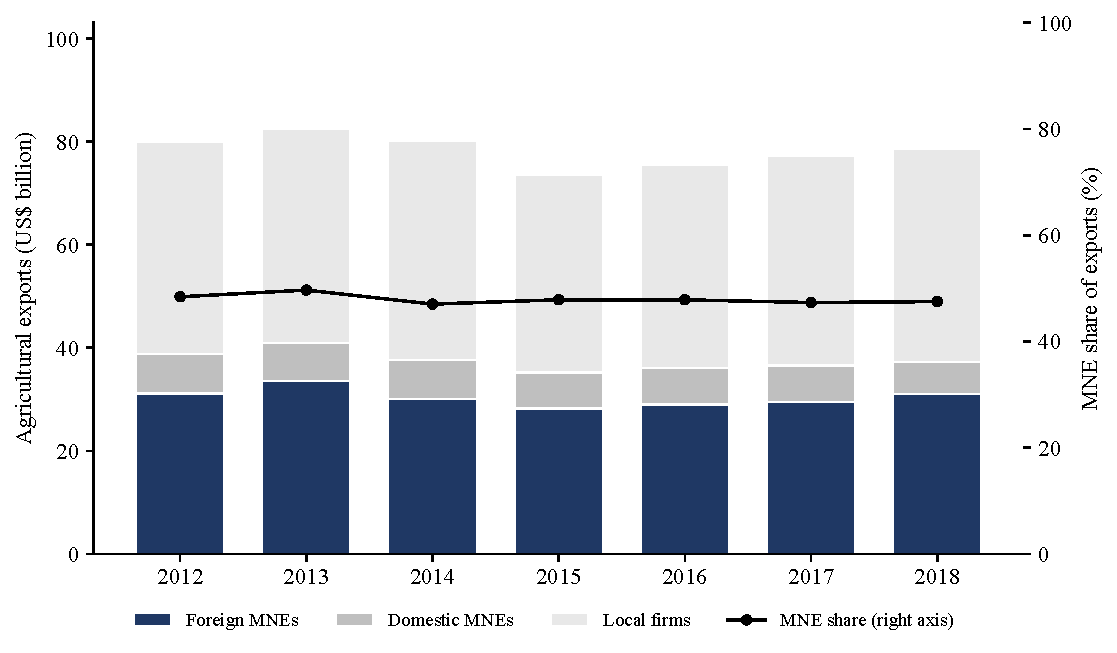
\includegraphics[width=0.85\textwidth,height=0.8\textheight,keepaspectratio]{figures/agro/fig_agp_trend.pdf}%
  \par\vspace{2pt}%
  \parbox{0.92\textwidth}{\footnotesize %
  \textit{Notes:} Agricultural exports (HS 01--24) of the nine countries. Bars: exports by type of exporter, in current US\$ billion. Line: share of MNE affiliates in the total (right axis).\\[3pt]%
  \srcnote}%
  \end{figure}

\subsubsection{Destinations}

The region sells its agricultural products to many markets, and the United States, Canada and
China gained weight over the period. Over 2012--2018, Latin America and the Caribbean took 27
percent of the exports, Europe 24 percent, Asia without China 18 percent, the United States and
Canada 15 percent, China 10 percent and Africa 6 percent (see Table~\ref{tab:dest}). Between 2012
and 2018, the share going to other Latin American countries fell from 29 to 26 percent, while the
share of the United States and Canada rose from 13 to 16 percent and that of China from 9 to 10
percent (see Figure~\ref{fig:trend_dest}).

The next figure shows how the destination of agricultural exports changed from year to year. Each
bar adds to 100 and shows the share of each destination region in that year
(see Figure~\ref{fig:trend_dest}).
% ---- Figure: Destination of Agricultural Exports, 2012--2018
\begin{figure}[H]\centering%
  \caption{Destination of Agricultural Exports, 2012--2018}%
  \label{fig:trend_dest}%
  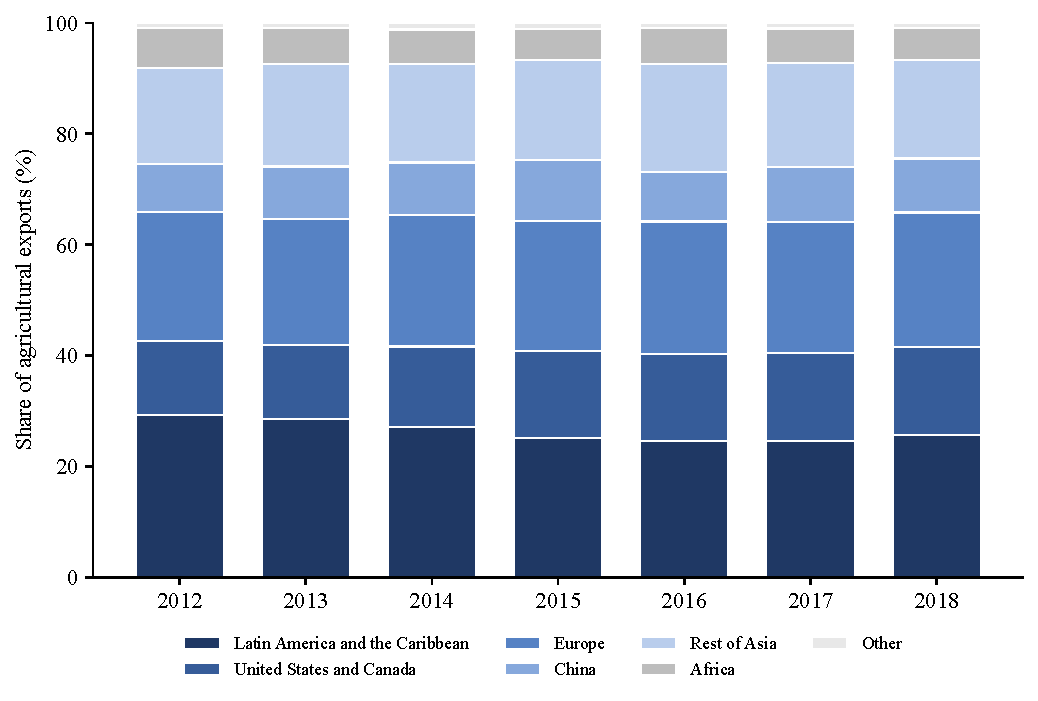
\includegraphics[width=0.85\textwidth,height=0.8\textheight,keepaspectratio]{figures/agro/fig_agp_trend_dest.pdf}%
  \par\vspace{2pt}%
  \parbox{0.92\textwidth}{\footnotesize %
  \textit{Notes:} Shares of the agricultural exports of the nine countries, by destination region. China includes Hong Kong and Macao. Europe includes countries outside the European Union; Rest of Asia includes the Middle East.\\[3pt]%
  \srcnote}%
  \end{figure}

Foreign affiliates are more present in exports to some markets than to others. They ship 47
percent of the exports that go to other Latin American countries and 45 percent of those that go
to China, against 34 and 33 percent of those that go to North America and Europe. The next table
shows, for each destination region, its share of total exports and the share shipped by each type
of exporter (see Table~\ref{tab:dest}).
% ---- Table: Agricultural Exports and Ownership, by Destination Region
\begin{table}[H]\centering\small%
  \caption{Agricultural Exports and Ownership, by Destination Region}%
  \label{tab:dest}%
  \adjustbox{max width=\textwidth, max totalheight=0.8\textheight}{\begin{tabular}{lrrrrr}
\toprule
Destination & Share of exports (\%) & Foreign MNEs (\%) & Domestic MNEs (\%) & Local firms (\%) & Exports (US\$bn/yr) \\
\midrule
Latin America and the Caribbean & 26.5 & 46.9 & 7.4 & 45.7 & 20.7 \\
United States and Canada & 14.8 & 33.9 & 8.4 & 57.7 & 11.6 \\
Europe & 23.6 & 33.0 & 7.7 & 59.3 & 18.4 \\
China & 9.6 & 44.6 & 8.9 & 46.5 & 7.5 \\
Rest of Asia & 18.2 & 36.7 & 13.2 & 50.1 & 14.2 \\
Africa & 6.3 & 38.1 & 12.2 & 49.7 & 4.9 \\
Other & 1.0 & 23.7 & 10.3 & 66.1 & 0.8 \\
\midrule
All destinations & 100.0 & 38.8 & 9.1 & 52.0 & 78.2 \\
\bottomrule
\end{tabular}
}%
  \par\vspace{3pt}%
  \begin{minipage}{0.95\textwidth}\footnotesize %
  \textit{Notes:} Column (1): percent of the agricultural exports of the nine countries going to each region. Columns (2)--(4): percent of the exports to each region shipped by each type of exporter. Exports are annual averages over 2012--2018, in US\$ billion.\\[3pt]%
  \srcnote%
  \end{minipage}%
  \end{table}

\subsubsection{Exporters}

Multinational affiliates are a fifth of agricultural exporters, and they are larger and sell to
more markets than local firms. Foreign affiliates are 17 percent of exporters and ship 39 percent
of the value, while local firms are 80 percent of exporters and ship 52 percent (see
Table~\ref{tab:firms}). In an average year, a foreign or a domestic affiliate exports about
US\$11.5 million, almost three times as much as a local firm (US\$4.2 million). Affiliates also
reach more destinations, 5.3 (foreign) and 6.0 (domestic) on average against 3.8 for local firms,
while the number of products per firm is similar in the three groups.

The next table compares the three types of exporters. It shows their number, their share of
exporters and of export value, and the average value, number of products and number of
destinations per firm and year (see Table~\ref{tab:firms}).
% ---- Table: Agricultural Exporters, by Type of Owner
\begin{table}[H]\centering\small%
  \caption{Agricultural Exporters, by Type of Owner}%
  \label{tab:firms}%
  \adjustbox{max width=\textwidth, max totalheight=0.8\textheight}{\begin{tabular}{lrrrr}
\toprule
 & Foreign MNEs & Domestic MNEs & Local firms & All exporters \\
\midrule
Number of exporters & 5,166 & 1,164 & 24,528 & 30,858 \\
Share of exporters (\%) & 16.7 & 3.8 & 79.5 & 100.0 \\
Share of export value (\%) & 38.8 & 9.1 & 52.0 & 100.0 \\
Exports per firm and year, mean (US\$ million) & 11.53 & 11.46 & 4.18 & 6.01 \\
Exports per firm and year, median (US\$ million) & 0.443 & 0.511 & 0.168 & 0.215 \\
Products per firm and year, mean & 3.3 & 3.0 & 3.0 & 3.1 \\
Products per firm and year, median & 2 & 2 & 1 & 1 \\
Destinations per firm and year, mean & 5.3 & 6.0 & 3.8 & 4.3 \\
Destinations per firm and year, median & 2 & 2 & 2 & 2 \\
\bottomrule
\end{tabular}
}%
  \par\vspace{3pt}%
  \begin{minipage}{0.95\textwidth}\footnotesize %
  \textit{Notes:} Agricultural exporters of the nine countries, 2012--2018. Exporters are distinct tax identifiers within each country. Exports, products and destinations are computed for each firm and year and then averaged over all firm-years.\\[3pt]%
  \srcnote%
  \end{minipage}%
  \end{table}

\subsubsection{Products}

A few product groups make up most of the region's agricultural exports, and soybean products alone
account for more than a quarter. The largest groups are animal feed (US\$14.1 billion a year,
mostly soybean meal), vegetables and fruit (10.4), cereals (10.3), oil seeds (7.1) and vegetable
oils (5.8) (see Table~\ref{tab:sitc}). Soybean meal, soybeans and crude soybean oil together
amount to US\$21.8 billion a year, 28 percent of the total (see Figure~\ref{fig:hs6}).

The foreign share is highest in miscellaneous food products (71 percent), oil seeds (61 percent),
tobacco (55 percent) and cereals (48 percent), and lowest in sugar (21 percent) and in coffee,
beverages and dairy (about 30 percent each). Domestic multinationals are
most present in dairy (23 percent), sugar (18 percent) and coffee (16 percent). The main parent
countries also change from one group to another: US groups lead in oil seeds (54 percent of the
exports of foreign affiliates) and cereals (33 percent), Swiss and Liechtenstein groups in animal
feed (28 and 19 percent), German groups in coffee (42 percent), Saudi and Brazilian groups in meat,
and Spanish groups in fish and in vegetables and fruit. Agricultural inputs (seeds, animal feed
and live animals) and the other agricultural products have similar foreign shares, 36 and 40
percent (see Table~\ref{tab:ap_inputs} in the Appendix).

The share of multinationals does not follow a clear pattern with how sophisticated the product is.
The foreign share goes up and down across groups of products ranked by the Product Complexity
Index, and it is similar for differentiated goods and for goods traded on organized exchanges (43
and 41 percent). By end use, it is 42 percent for intermediate goods and 36 percent for consumer
goods. These results are in Appendix~\ref{sec:ap_soph}.

The next table splits agricultural exports into product groups. For each group, it shows the
value exported, the value shipped by multinationals, the foreign and domestic shares, and the
three parent countries with the largest shares of the group's foreign-affiliate exports (see
Table~\ref{tab:sitc}).
% ---- Table: Agricultural Exports and Multinational Shares, by Product Group
\begin{table}[H]\centering\footnotesize%
  \caption{Agricultural Exports and Multinational Shares, by Product Group}%
  \label{tab:sitc}%
  \adjustbox{max width=\textwidth, max totalheight=0.8\textheight}{\begin{tabular}{@{}l r r r r l@{}}
\toprule
SITC Rev.\,3 division & Total exports (US\$bn/yr) & MNE exports (US\$bn/yr) & Foreign (\%) & Domestic (\%) & Leading parents (share of foreign) \\
\midrule
08 Animal feed & 14.1 & 6.6 & 35.7 & 11.5 & CHE 0.28, LIE 0.19, USA 0.19 \\
05 Vegetables \& fruit & 10.4 & 4.0 & 33.2 & 5.1 & ESP 0.14, USA 0.13, PAN 0.12 \\
04 Cereals & 10.3 & 5.9 & 48.4 & 8.4 & USA 0.33, CHE 0.13, NLD 0.13 \\
22 Oil seeds & 7.1 & 4.6 & 60.5 & 3.9 & USA 0.54, NLD 0.13, LIE 0.09 \\
42 Fixed vegetable oils & 5.8 & 2.4 & 30.9 & 10.8 & CHE 0.25, NLD 0.25, USA 0.24 \\
07 Coffee, tea, cocoa, spices & 4.9 & 2.2 & 30.0 & 15.6 & DEU 0.42, ITA 0.13, SGP 0.10 \\
01 Meat & 4.7 & 2.1 & 34.0 & 10.4 & SAU 0.47, BRA 0.25, JPN 0.06 \\
03 Fish \& seafood & 3.3 & 1.8 & 46.2 & 7.5 & ESP 0.37, LUX 0.14, VEN 0.09 \\
11 Beverages & 2.2 & 0.8 & 29.5 & 7.6 & LUX 0.18, GBR 0.15, PAN 0.12 \\
29 Crude animal/veg. materials & 2.2 & 0.8 & 27.6 & 7.8 & DEU 0.10, ARG 0.10, CHL 0.08 \\
02 Dairy \& eggs & 1.9 & 0.9 & 27.7 & 22.9 & NLD 0.22, ROU 0.20, CHE 0.17 \\
09 Misc. edible products & 1.7 & 1.3 & 71.4 & 2.1 & USA 0.45, CHE 0.18, FRA 0.10 \\
06 Sugar \& honey & 1.4 & 0.5 & 21.4 & 17.9 & USA 0.51, KOR 0.19, LIE 0.14 \\
12 Tobacco & 1.2 & 0.7 & 54.5 & 0.1 & USA 0.36, HKG 0.27, KOR 0.11 \\
41 Animal oils \& fats & 0.5 & 0.2 & 21.9 & 9.6 & BMU 0.34, PAN 0.25, GBR 0.17 \\
Other & 0.5 & 0.1 & 24.3 & 2.2 & CHE 0.25, USA 0.21, GBR 0.08 \\
\midrule
All & 72.2 & 34.9 & 39.3 & 9.0 & \\
\bottomrule
\end{tabular}
}%
  \par\vspace{3pt}%
  \begin{minipage}{0.95\textwidth}\footnotesize %
  \textit{Notes:} Agricultural exports by SITC Rev.\,3 division, 2012--2018. Foreign and domestic: percent of the division's export value. Leading parents: the three largest parent countries and their share of the division's foreign-MNE exports. Values are annual averages in US\$ billion. Products without an SITC correspondence (US\$6.0 billion a year) are excluded.\\[3pt]%
  \srcnote%
  \end{minipage}%
  \end{table}

The next figure looks at the twenty largest agricultural products. For each product, it shows the
share shipped by foreign multinationals, domestic multinationals and local firms (see
Figure~\ref{fig:hs6}).
% ---- Figure: Ownership of the Twenty Largest Agricultural Export Products
\begin{figure}[H]\centering%
  \caption{Ownership of the Twenty Largest Agricultural Export Products}%
  \label{fig:hs6}%
  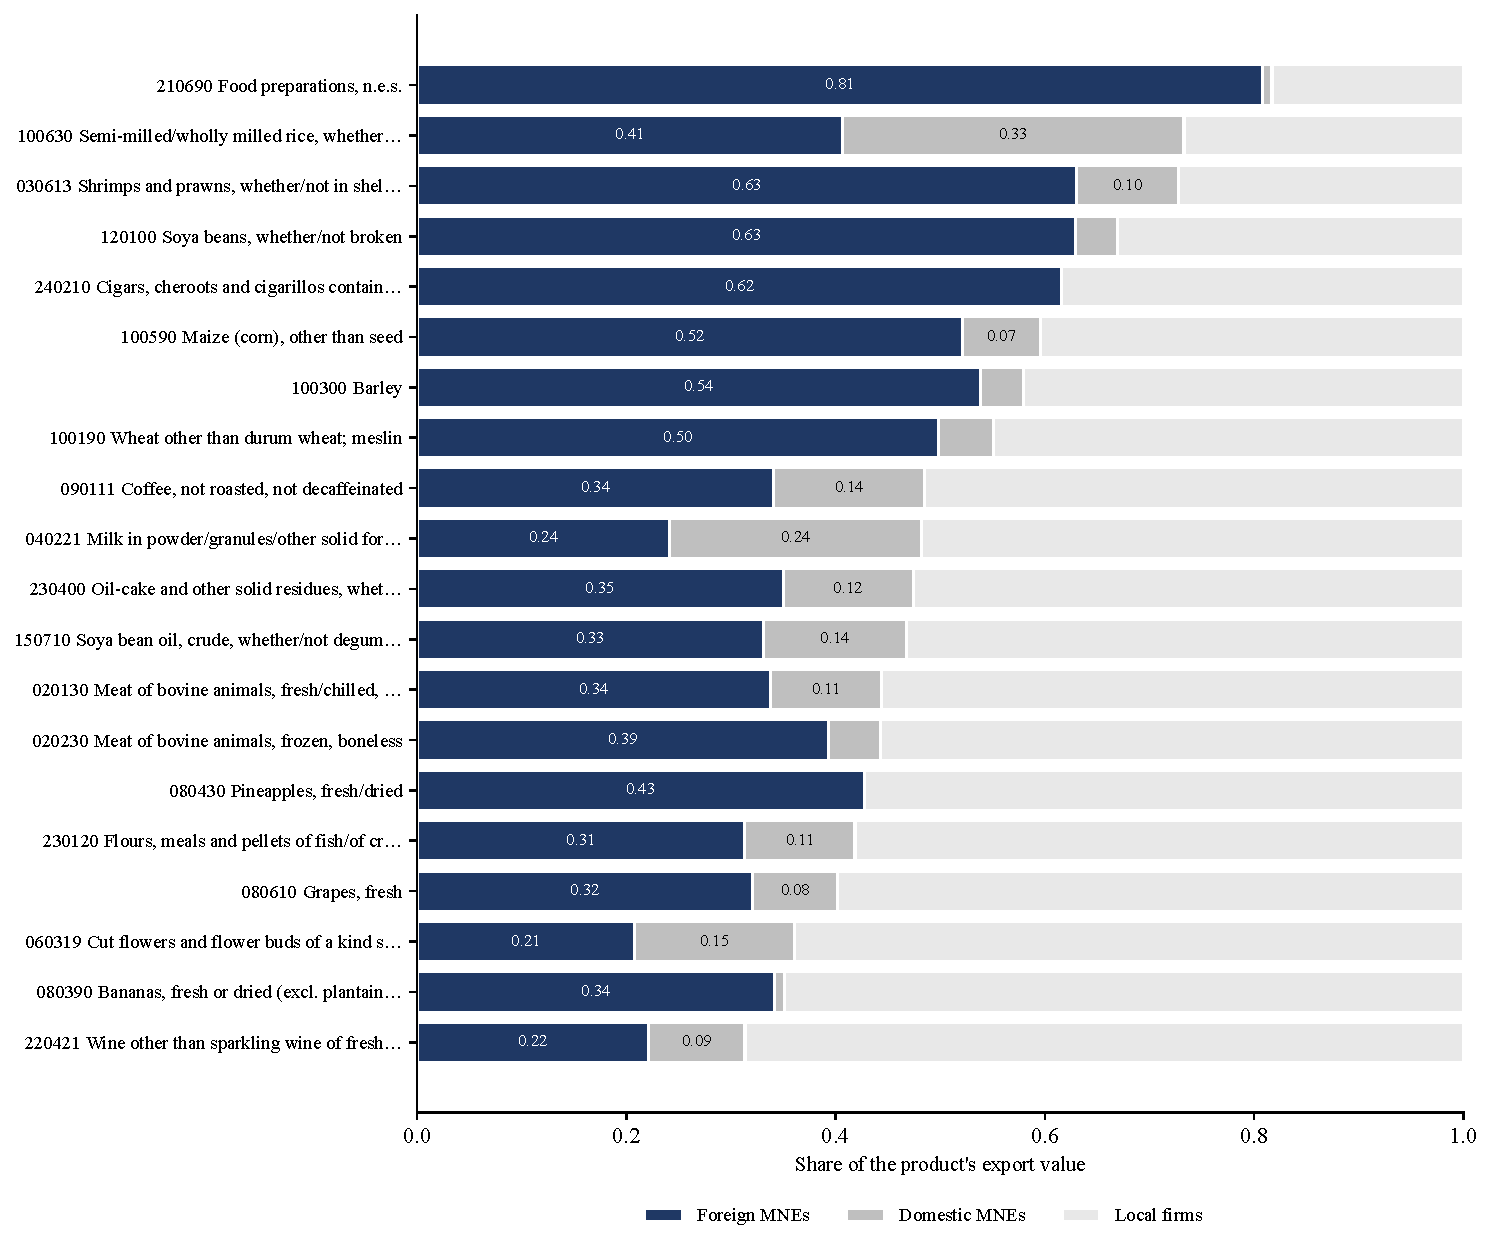
\includegraphics[width=1.0\textwidth,height=0.8\textheight,keepaspectratio]{figures/agro/fig_wp1f_top20_hs6_stacked.pdf}%
  \par\vspace{2pt}%
  \parbox{0.92\textwidth}{\footnotesize %
  \textit{Notes:} Shares of each product's export value, by type of exporter, 2012--2018. The twenty largest agricultural products by export value.\\[3pt]%
  \srcnote}%
  \end{figure}

%======================================================================
\section{Who Owns Agricultural Exports}\label{sec:owners}
%======================================================================
\subsection{Multinationals Ship Almost Half of Agricultural Exports}

Multinational firms ship 48 percent of the agricultural exports of the nine countries, 39 percent
through foreign affiliates and 9 percent through domestic ones (see Figure~\ref{fig:f1}). The share
is highest in Paraguay (66 percent) and Uruguay (63 percent), the two countries where agriculture
weighs most in exports, and lowest in Peru (38 percent) and El Salvador (30 percent). Foreign
affiliates ship more than domestic ones in every country. The gap is smallest in Chile (30 against
18 percent) and Colombia (28 against 15 percent), where domestic groups are larger.

The next figure shows the share of each country's agricultural exports shipped by foreign and
domestic multinationals. The last bar, LAC9, is the nine countries together (see
Figure~\ref{fig:f1}).
% ---- Figure: Multinational Share of Agricultural Exports, by Exporting Country
\begin{figure}[H]\centering%
  \caption{Multinational Share of Agricultural Exports, by Exporting Country}%
  \label{fig:f1}%
  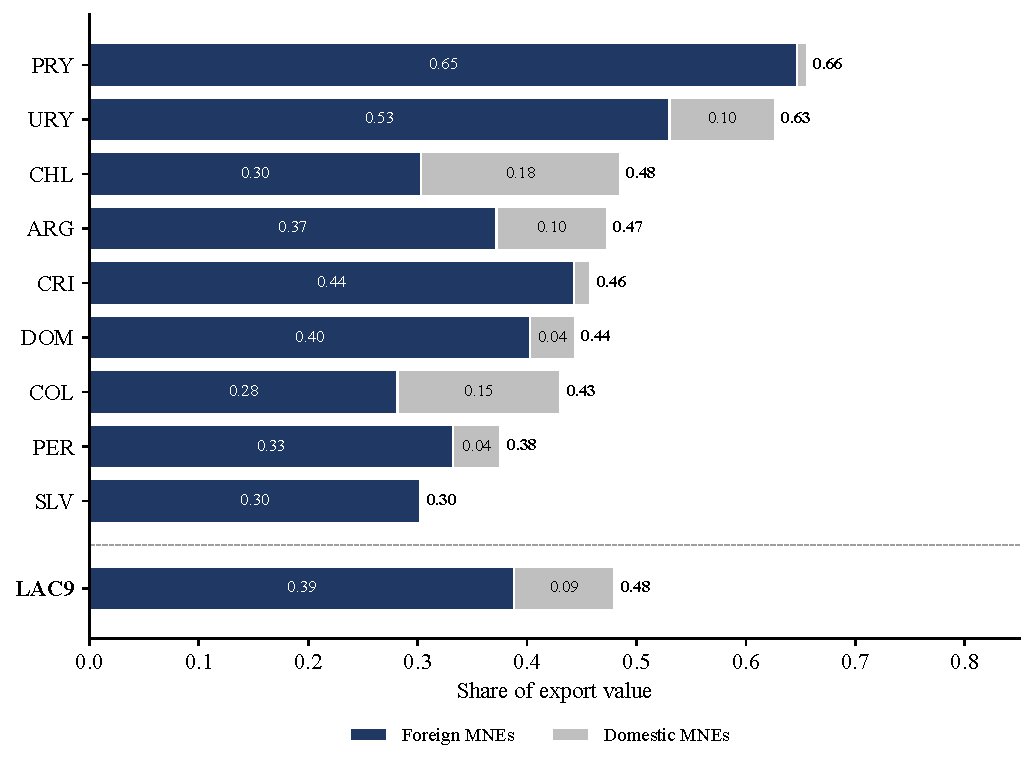
\includegraphics[width=0.8\textwidth,height=0.8\textheight,keepaspectratio]{figures/agro/fig_agp_origin_lac9.pdf}%
  \par\vspace{2pt}%
  \parbox{0.92\textwidth}{\footnotesize %
  \textit{Notes:} Shares of agricultural export value (HS 01--24), 2012--2018 pooled. LAC9: the nine countries together. The number at the end of each bar is the total MNE share.\\[3pt]%
  \srcnote}%
  \end{figure}

\subsection{Parents Are Based in a Few Countries}

The parents of foreign affiliates are based in a few countries, and more than a quarter of foreign
ownership is recorded in tax havens. Among the countries that are not tax havens, the United States
accounts for 25 percent of the exports of foreign affiliates and the Netherlands for 10 percent; no
other country reaches 5 percent (see Figure~\ref{fig:parents}, Panel A). Tax havens and similar
jurisdictions account for 29 percent together, led by Switzerland (11 percent), Liechtenstein (8
percent), Luxembourg (3 percent) and Panama (2 percent) (Panel B). Almost all of the Swiss and
Liechtenstein shares come from exporters in Argentina. Where the exports of each parent country go
is shown in Tables~\ref{tab:ap_pxd} and~\ref{tab:ap_pxp} in the Appendix.

The next figure ranks parent countries by their share of the agricultural exports of foreign
affiliates. Panel A shows countries that are not tax havens and Panel B shows tax havens (see
Figure~\ref{fig:parents}).
% ---- Figure: Foreign-Multinational Agricultural Exports, by Parent Country
\begin{figure}[H]\centering%
  \caption{Foreign-Multinational Agricultural Exports, by Parent Country}%
  \label{fig:parents}%
  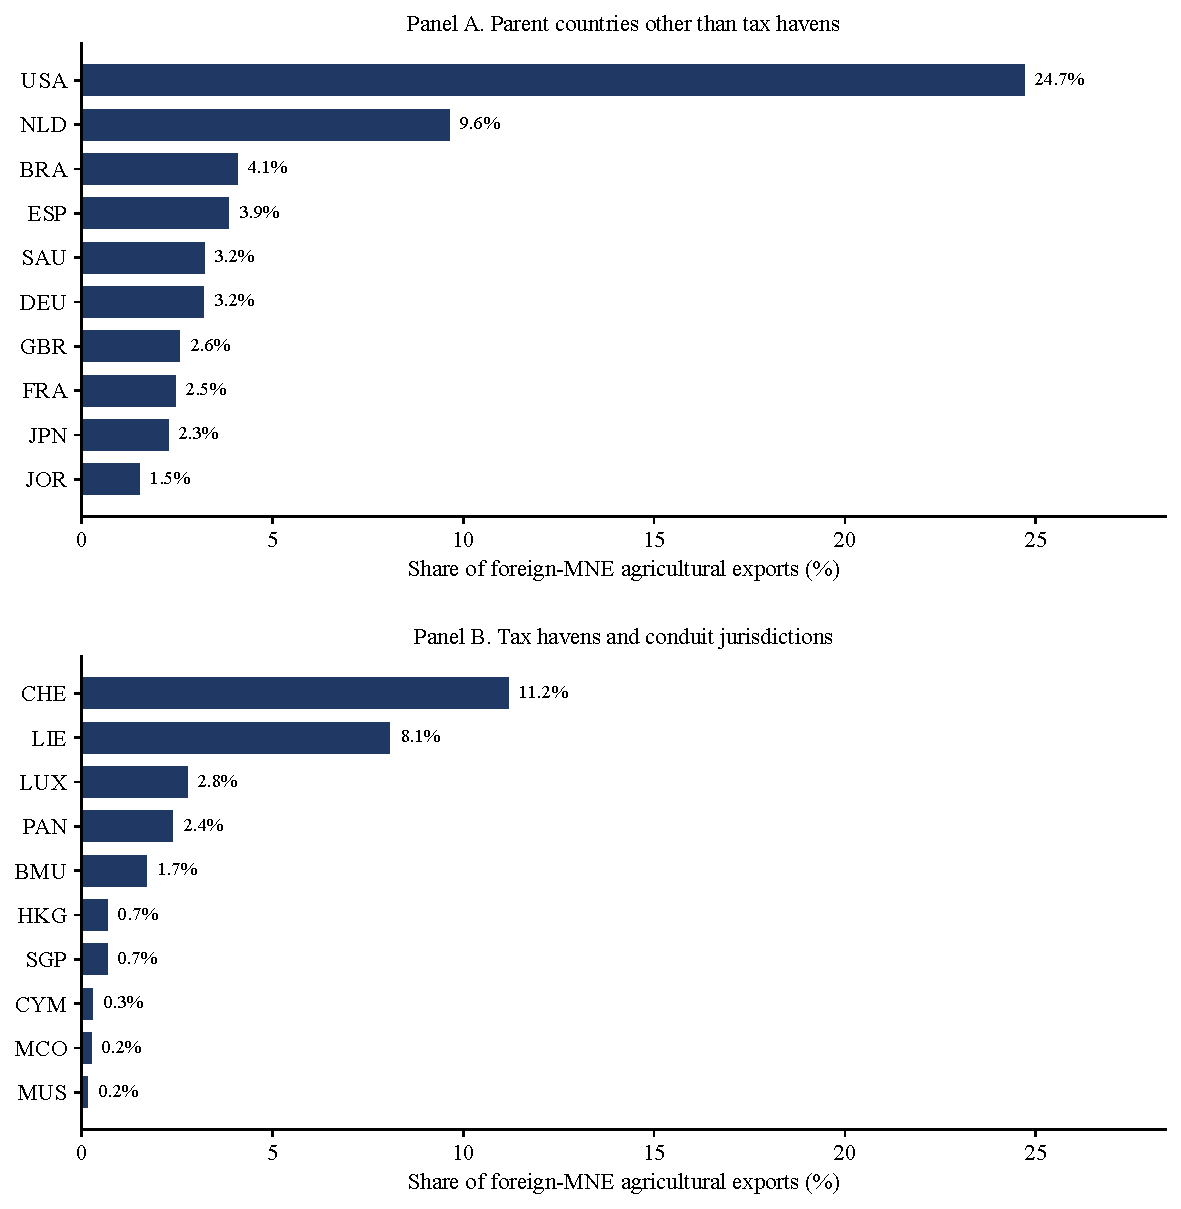
\includegraphics[width=0.8\textwidth,height=0.8\textheight,keepaspectratio]{figures/agro/fig_agp_parent_panels.pdf}%
  \par\vspace{2pt}%
  \parbox{0.92\textwidth}{\footnotesize %
  \textit{Notes:} Percent of the agricultural exports of foreign MNEs with a recorded parent country (89 percent of the total), by country of the ultimate parent, 2012--2018. The ten largest in each panel. Panel A: parent countries that are not tax havens. Panel B: tax havens and conduit jurisdictions (Switzerland, Liechtenstein, Luxembourg, Panama, Ireland, Singapore, the United Arab Emirates, small island economies and dependent territories such as Bermuda, the Cayman Islands and Hong Kong).\\[3pt]%
  \srcnote}%
  \end{figure}

\subsection{A Few Large Groups Ship Most Foreign-Affiliate Exports}

Most of the exports of foreign affiliates come from groups with very large networks. In
agriculture, 44 percent of parents have only one affiliate in the world, but the 13 percent with
more than 100 affiliates ship half of the exports of foreign affiliates (see
Figure~\ref{fig:network}). Groups with 11 to 100 affiliates ship another 30 percent, so groups with
more than ten affiliates account for 80 percent of the total.

The next figure groups parents by the number of affiliates they have worldwide. For each size
group, it shows the share of parents and the share of the exports of foreign affiliates (see
Figure~\ref{fig:network}).
% ---- Figure: Foreign-Multinational Agricultural Exports and Number of Parents, by Size of the Group's Global Network
\begin{figure}[H]\centering%
  \caption{Foreign-Multinational Agricultural Exports and Number of Parents, by Size of the Group's Global Network}%
  \label{fig:network}%
  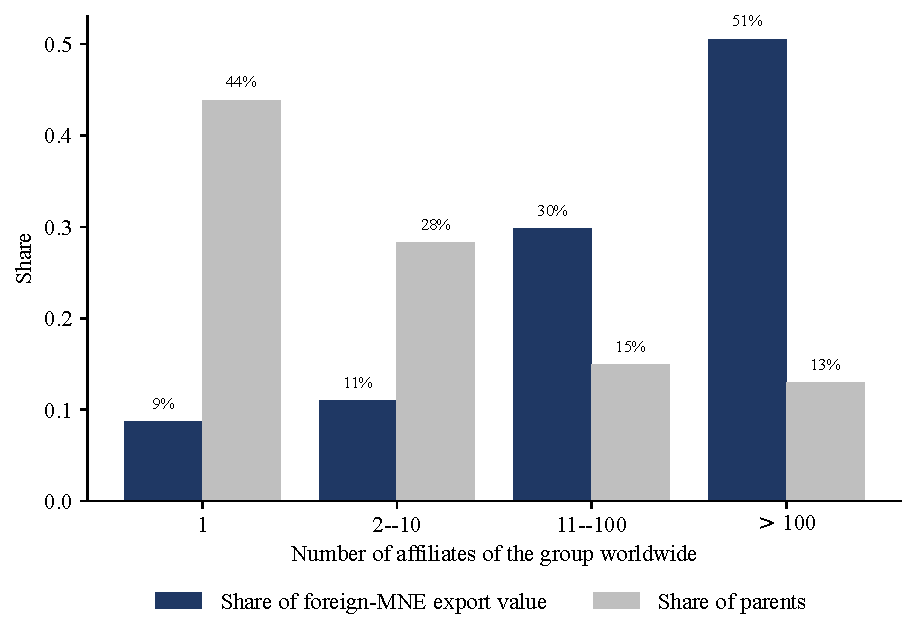
\includegraphics[width=0.7\textwidth,height=0.8\textheight,keepaspectratio]{figures/agro/fig_wp0_fig5_network.pdf}%
  \par\vspace{2pt}%
  \parbox{0.92\textwidth}{\footnotesize %
  \textit{Notes:} Shares of foreign-MNE agricultural export value and of parents, by the number of affiliates the group has worldwide, 2012--2018.\\[3pt]%
  \srcnote}%
  \end{figure}

%======================================================================
\section{Multinationals and Export Performance}\label{sec:perf}
%======================================================================
\subsection{Multinational Presence and Exports}

To see whether exports are larger where more multinational firms are present, we estimate a
regression at the origin country ($o$), destination country ($d$), product ($p$) and year ($y$)
level:
\begin{equation}\label{eq:presence}
\ln X_{odpy} = \beta \ln N_{odpy} + \delta_{odp} + \delta_{ody} + \varepsilon_{odpy},
\end{equation}
where $X_{odpy}$ is the value of product $p$ exported from country $o$ to country $d$ in year
$y$, and $N_{odpy}$ is the number of multinational firms that export it. We first estimate this
equation using only the observations with at least one multinational firm; this is the
\emph{intensive margin}. We then replace $\ln N_{odpy}$ with a variable equal to one if at least
one multinational firm exports the product from $o$ to $d$ in year $y$; this is the
\emph{extensive margin}. In the strictest version, $\delta_{odp}$ and $\delta_{ody}$ are fixed
effects for each origin--destination--product and each origin--destination--year. They absorb,
for example, the fact that some countries export some products to some markets every year, and
changes over time in the trade costs between two countries. Other columns use fewer fixed effects.
We also estimate the equation with the exports of local firms only as the dependent variable.
Standard errors are clustered by origin--destination pair. The regression describes correlations;
it does not separate the effect of multinational firms from their choice of where to operate.

Exports are larger where more multinational firms are present, and so are the exports of local
firms. With the strictest fixed effects, a 10 percent increase in the number of multinationals
that export a product from a country to a destination in a given year is associated with about 8
percent higher exports, and having at least one multinational is associated with exports about 90
percent higher (see Table~\ref{tab:t1}, column 3 of each margin). Local firms also export more
where multinationals are present: the elasticity is 0.37, and their exports are 27 percent higher
when at least one multinational is present (Panel B).

The next table reports the estimates of equation~(\ref{eq:presence}). Panel A uses total exports
and Panel B the exports of local firms only. The first three columns give the intensive margin and
the last three the extensive margin, each with three sets of fixed effects (see
Table~\ref{tab:t1}).
% ---- Table: Multinational Presence and Agricultural Exports
\begin{table}[H]\centering\small%
  \caption{Multinational Presence and Agricultural Exports}%
  \label{tab:t1}%
  \adjustbox{max width=\textwidth, max totalheight=0.8\textheight}{\begin{tabular}{lcccccc} \hline
 & \multicolumn{3}{c}{Intensive: $\ln$(\# MNE firms)} & \multicolumn{3}{c}{Extensive: any MNE present} \\
 & (1) & (2) & (3) & (1) & (2) & (3) \\ \hline
\multicolumn{7}{l}{\textit{Panel A. Dependent variable: $\ln$ exports, all firms}} \\
$\ln$(\# MNE firms) & 2.2005*** & 2.2049*** & 0.7969*** &  &  &  \\
 & (0.0288) & (0.0286) & (0.0219) &  &  &  \\
Any MNE present &  &  &  & 1.8183*** & 1.8195*** & 0.6549*** \\
 &  &  &  & (0.0652) & (0.0647) & (0.0262) \\
\midrule
\multicolumn{7}{l}{\textit{Panel B. Dependent variable: $\ln$ exports, local firms}} \\
$\ln$(\# MNE firms) & 1.5784*** & 1.5891*** & 0.3746*** &  &  &  \\
 & (0.0351) & (0.0352) & (0.0280) &  &  &  \\
Any MNE present &  &  &  & 1.9466*** & 1.9479*** & 0.2390*** \\
 &  &  &  & (0.0640) & (0.0628) & (0.0210) \\
\hline
Origin FE & $\checkmark$ &  &  & $\checkmark$ &  &  \\
Destination FE & $\checkmark$ &  &  & $\checkmark$ &  &  \\
Product FE & $\checkmark$ & $\checkmark$ &  & $\checkmark$ & $\checkmark$ &  \\
Year FE & $\checkmark$ &  &  & $\checkmark$ &  &  \\
Origin $\times$ year FE &  & $\checkmark$ &  &  & $\checkmark$ &  \\
Destination $\times$ year FE &  & $\checkmark$ &  &  & $\checkmark$ &  \\
Origin $\times$ dest.\ $\times$ product FE &  &  & $\checkmark$ &  &  & $\checkmark$ \\
Origin $\times$ dest.\ $\times$ year FE &  &  & $\checkmark$ &  &  & $\checkmark$ \\
Observations (Panel A) & 101,098 & 100,983 & 88,037 & 198,231 & 198,142 & 175,847 \\
Observations (Panel B) & 59,848 & 59,708 & 52,515 & 156,990 & 156,915 & 137,240 \\
\hline
\end{tabular}
}%
  \par\vspace{3pt}%
  \begin{minipage}{0.95\textwidth}\footnotesize %
  \textit{Notes:} Regression at the origin country, destination country, product and year level; agricultural products, 2012--2018. Dependent variable: $\ln$ exports (Panel A) and $\ln$ exports of local firms (Panel B). Intensive margin: $\ln$ number of MNEs, observations with at least one MNE. Extensive margin: indicator for at least one MNE. Standard errors clustered by origin--destination pair in parentheses. *** $p<0.01$, ** $p<0.05$, * $p<0.1$.\\[3pt]%
  \srcnote%
  \end{minipage}%
  \end{table}

The link is stronger for foreign multinationals than for domestic ones. With the strictest fixed
effects, the elasticity is 0.46 for foreign affiliates and 0.24 for domestic ones (see
Table~\ref{tab:counts}, column 4). Among foreign affiliates, the elasticity is larger for those
exporting to countries other than the parent's country (0.37 against 0.24, column 6).

The next table repeats the intensive margin, splitting the number of multinationals into foreign
and domestic affiliates (columns 3 and 4), and then splitting foreign affiliates by whether the
destination is the parent's country (columns 5 and 6) (see Table~\ref{tab:counts}).
% ---- Table: Multinational Presence and Agricultural Exports, by Type of Multinational
\begin{table}[H]\centering\small%
  \caption{Multinational Presence and Agricultural Exports, by Type of Multinational}%
  \label{tab:counts}%
  \adjustbox{max width=\textwidth, max totalheight=0.8\textheight}{\begin{tabular}{lcccccc} \hline
 & \multicolumn{2}{c}{All MNEs} & \multicolumn{2}{c}{Foreign / domestic} & \multicolumn{2}{c}{Foreign by destination, domestic} \\
 & (1) & (2) & (3) & (4) & (5) & (6) \\ \hline
\multicolumn{7}{l}{\textit{Panel A. Dependent variable: $\ln$ exports, all firms}} \\
$\ln$(\# MNE firms) & 2.2049*** & 0.7969*** &  &  &  &  \\
 & (0.0286) & (0.0219) &  &  &  &  \\
$\ln$(\# foreign MNEs) &  &  & 1.3461*** & 0.4555*** &  &  \\
 &  &  & (0.0298) & (0.0234) &  &  \\
$\ln$(\# foreign MNEs, parent-country destination) &  &  &  &  & 0.4122*** & 0.2425** \\
 &  &  &  &  & (0.1311) & (0.0905) \\
$\ln$(\# foreign MNEs, other destinations) &  &  &  &  & 0.9464*** & 0.3662*** \\
 &  &  &  &  & (0.0791) & (0.0417) \\
$\ln$(\# domestic MNEs) &  &  & 0.4836*** & 0.2434*** & 0.3740*** & 0.1957*** \\
 &  &  & (0.0321) & (0.0216) & (0.0806) & (0.0616) \\
\midrule
\multicolumn{7}{l}{\textit{Panel B. Dependent variable: $\ln$ exports, local firms}} \\
$\ln$(\# MNE firms) & 1.5891*** & 0.3746*** &  &  &  &  \\
 & (0.0352) & (0.0280) &  &  &  &  \\
$\ln$(\# foreign MNEs) &  &  & 1.2729*** & 0.3421*** &  &  \\
 &  &  & (0.0412) & (0.0343) &  &  \\
$\ln$(\# foreign MNEs, parent-country destination) &  &  &  &  & 0.3480** & 0.3453*** \\
 &  &  &  &  & (0.1599) & (0.0986) \\
$\ln$(\# foreign MNEs, other destinations) &  &  &  &  & 1.2094*** & 0.4941*** \\
 &  &  &  &  & (0.1295) & (0.1352) \\
$\ln$(\# domestic MNEs) &  &  & 0.5358*** & 0.2428*** & 0.3675** & 0.2183** \\
 &  &  & (0.0463) & (0.0304) & (0.1509) & (0.1042) \\
\hline
Product FE & $\checkmark$ &  & $\checkmark$ &  & $\checkmark$ &  \\
Origin $\times$ year FE & $\checkmark$ &  & $\checkmark$ &  & $\checkmark$ &  \\
Destination $\times$ year FE & $\checkmark$ &  & $\checkmark$ &  & $\checkmark$ &  \\
Origin $\times$ dest.\ $\times$ product FE &  & $\checkmark$ &  & $\checkmark$ &  & $\checkmark$ \\
Origin $\times$ dest.\ $\times$ year FE &  & $\checkmark$ &  & $\checkmark$ &  & $\checkmark$ \\
Observations (Panel A) & 100,983 & 88,037 & 15,517 & 13,103 & 1,179 & 938 \\
Observations (Panel B) & 59,708 & 52,515 & 13,728 & 11,643 & 1,150 & 922 \\
\hline
\end{tabular}
}%
  \par\vspace{3pt}%
  \begin{minipage}{0.95\textwidth}\footnotesize %
  \textit{Notes:} Regression at the origin country, destination country, product and year level; agricultural products, 2012--2018. Dependent variable: $\ln$ exports (Panel A) and $\ln$ exports of local firms (Panel B). Regressors: $\ln$ number of MNEs of each type. Columns (5)--(6) split foreign MNEs by whether the destination is the parent's country. Standard errors clustered by origin--destination pair in parentheses. *** $p<0.01$, ** $p<0.05$, * $p<0.1$.\\[3pt]%
  \srcnote%
  \end{minipage}%
  \end{table}

\subsection{Distance}

To see whether distance reduces the exports of multinational firms less than those of local firms,
we estimate a regression at the firm ($f$), destination country ($d$), product ($p$) and year ($y$)
level:
\begin{equation}\label{eq:dist}
\ln x_{fdpy} = \alpha \ln D_{od} + \gamma \left(M_{f} \times \ln D_{od}\right) + \delta_{oy} + \delta_{dy} + \delta_{p} + u_{fdpy},
\end{equation}
where $x_{fdpy}$ is the value of product $p$ exported by firm $f$, located in country $o$, to
country $d$ in year $y$; $D_{od}$ is the distance between the two countries, from the CEPII
gravity database; and $M_f$ equals one if the firm is a multinational affiliate. The coefficient
$\alpha$ measures how exports fall with distance for local firms, and $\gamma$ shows how much
smaller this effect is for multinationals. The fixed effects $\delta_{oy}$, $\delta_{dy}$ and
$\delta_p$ absorb changes over time in each origin and each destination and differences across
products; other columns use origin, destination and year fixed effects instead. We also split
multinationals by whether the group is present in the destination (it has an affiliate there, or
the destination is the parent's country) and into foreign and domestic multinationals. Standard
errors are clustered by origin--destination pair. As before, the regression describes
correlations.

Distance reduces the agricultural exports of multinational firms less than those of local firms.
For a local firm, exports fall by about 0.21 to 0.22 percent for each 1 percent of distance (see
Table~\ref{tab:t2}). This effect is about 15 percent smaller for multinationals and about 40
percent smaller when the group has an affiliate in the destination or the destination is the
parent's country (columns 3 and 4).

The next table reports the estimates of equation~(\ref{eq:dist}). Columns 1 and 2 compare all
multinationals with local firms. Columns 3 and 4 split multinationals by whether the group is
present in the destination (see Table~\ref{tab:t2}).
% ---- Table: Distance and Firm Agricultural Exports: Multinationals by Presence at the Destination
\begin{table}[H]\centering\small%
  \caption{Distance and Firm Agricultural Exports: Multinationals by Presence at the Destination}%
  \label{tab:t2}%
  \adjustbox{max width=\textwidth, max totalheight=0.8\textheight}{\begin{tabular}{lcccc} \hline
Dep.\ var.: $\ln$ exports & (1) & (2) & (3) & (4) \\ \hline
$\ln$ distance & -0.2115*** & -0.2217*** & -0.2072*** & -0.2173*** \\
 & (0.0805) & (0.0773) & (0.0802) & (0.0770) \\
$\ln$ distance $\times$ MNE & 0.0339*** & 0.0335*** &  &  \\
 & (0.0035) & (0.0035) &  &  \\
$\ln$ distance $\times$ MNE, present at destination &  &  & 0.0871*** & 0.0865*** \\
 &  &  & (0.0076) & (0.0076) \\
$\ln$ distance $\times$ MNE, not present at destination &  &  & 0.0246*** & 0.0243*** \\
 &  &  & (0.0036) & (0.0036) \\
\hline
Origin FE & $\checkmark$ &  & $\checkmark$ &  \\
Destination FE & $\checkmark$ &  & $\checkmark$ &  \\
Year FE & $\checkmark$ &  & $\checkmark$ &  \\
Origin $\times$ year FE &  & $\checkmark$ &  & $\checkmark$ \\
Destination $\times$ year FE &  & $\checkmark$ &  & $\checkmark$ \\
Product FE & $\checkmark$ & $\checkmark$ & $\checkmark$ & $\checkmark$ \\
\hline
Observations & 693,518 & 693,447 & 693,518 & 693,447 \\
\hline
\end{tabular}
}%
  \par\vspace{3pt}%
  \begin{minipage}{0.95\textwidth}\footnotesize %
  \textit{Notes:} Regression at the firm, destination country, product and year level; agricultural products, 2012--2018. Dependent variable: $\ln$ exports. Local firms are the omitted group. Present: the group has an affiliate in the destination or the destination is the parent's country. Standard errors clustered by origin--destination pair in parentheses. *** $p<0.01$, ** $p<0.05$, * $p<0.1$.\\[3pt]%
  \srcnote%
  \end{minipage}%
  \end{table}

The smaller effect of distance is stronger for foreign multinationals than for domestic ones. The
difference with local firms is 0.038 for foreign affiliates and 0.020 for domestic ones, so
distance reduces the exports of foreign affiliates about 17 percent less than those of local
firms, and those of domestic ones about 9 percent less (see Table~\ref{tab:dist}).

The next table splits multinationals into foreign and domestic affiliates (columns 1 and 2), and
then splits foreign affiliates by whether the destination is the parent's country (columns 3 and
4) (see Table~\ref{tab:dist}).
% ---- Table: Distance and Firm Agricultural Exports: Foreign and Domestic Multinationals
\begin{table}[H]\centering\small%
  \caption{Distance and Firm Agricultural Exports: Foreign and Domestic Multinationals}%
  \label{tab:dist}%
  \adjustbox{max width=\textwidth, max totalheight=0.8\textheight}{\begin{tabular}{lcccc} \hline
Dep.\ var.: $\ln$ exports & (1) & (2) & (3) & (4) \\ \hline
$\ln$ distance & -0.2129*** & -0.2230*** & -0.2123*** & -0.2224*** \\
 & (0.0805) & (0.0773) & (0.0805) & (0.0772) \\
$\ln$ distance $\times$ foreign MNE & 0.0375*** & 0.0371*** &  &  \\
 & (0.0037) & (0.0037) &  &  \\
$\ln$ distance $\times$ foreign MNE, parent-country destination &  &  & 0.0646*** & 0.0648*** \\
 &  &  & (0.0174) & (0.0173) \\
$\ln$ distance $\times$ foreign MNE, other destination &  &  & 0.0367*** & 0.0363*** \\
 &  &  & (0.0037) & (0.0037) \\
$\ln$ distance $\times$ domestic MNE & 0.0199*** & 0.0198*** & 0.0199*** & 0.0198*** \\
 & (0.0052) & (0.0052) & (0.0052) & (0.0052) \\
\hline
Origin FE & $\checkmark$ &  & $\checkmark$ &  \\
Destination FE & $\checkmark$ &  & $\checkmark$ &  \\
Year FE & $\checkmark$ &  & $\checkmark$ &  \\
Origin $\times$ year FE &  & $\checkmark$ &  & $\checkmark$ \\
Destination $\times$ year FE &  & $\checkmark$ &  & $\checkmark$ \\
Product FE & $\checkmark$ & $\checkmark$ & $\checkmark$ & $\checkmark$ \\
\hline
Observations & 693,518 & 693,447 & 693,518 & 693,447 \\
\hline
\end{tabular}
}%
  \par\vspace{3pt}%
  \begin{minipage}{0.95\textwidth}\footnotesize %
  \textit{Notes:} Regression at the firm, destination country, product and year level; agricultural products, 2012--2018. Dependent variable: $\ln$ exports. Local firms are the omitted group. Columns (3)--(4) split foreign MNEs by whether the destination is the parent's country. Standard errors clustered by origin--destination pair in parentheses. *** $p<0.01$, ** $p<0.05$, * $p<0.1$.\\[3pt]%
  \srcnote%
  \end{minipage}%
  \end{table}

%======================================================================
\section{Conclusion}\label{sec:concl}
%======================================================================
In this paper, we combine customs data from nine Latin American countries with ownership data from
Orbis and Dun \& Bradstreet to study the role of multinational firms in the region's agricultural
exports over 2012--2018. Multinational firms ship almost half of these exports, 39 percent
through foreign affiliates and 9 percent through domestic ones. This share stayed between 47 and
50 percent every year, while export values went up and down with commodity prices. It is highest
in Paraguay and Uruguay and lowest in Peru and El Salvador. Multinational affiliates are only a
fifth of agricultural exporters, but they export almost three times as much as local firms and
reach more markets.

Ownership is concentrated. A few parent countries, led by the United States and the Netherlands,
and a small number of groups with more than 100 affiliates worldwide account for most of the
exports of foreign affiliates, and more than a quarter of these exports belongs to groups whose
parent is recorded in a tax haven. Exports are larger where more multinational firms are present,
and the same holds for the exports of local firms. Distance is also a smaller barrier for the
exports of multinational firms, especially when the group already has an affiliate in the
destination country.

These results suggest three implications for policy, considering that they describe correlations
instead of causal effects. First, foreign investment and agricultural exports are closely linked
in the region, so policies that attract foreign investment are also export policies. Investment
promotion agencies can help countries attract multinational firms, mainly by reducing information
barriers (Harding and Javorcik, 2011; Volpe Martincus et al., 2021; Carballo, Marra de Arti\~nano
and Volpe Martincus, 2026). Second, local firms ship half of agricultural exports but are smaller
and reach fewer markets. Programs that help them sell to multinational firms could extend the
benefits of foreign presence: local firms that start supplying a multinational grow
(Alfaro-Ure\~na, Manelici and Vasquez, 2022) and are more likely to start exporting (Carballo et
al., 2021). Export promotion can also help them reach new markets and products (Volpe Martincus
and Carballo, 2008). Third, because a few large groups and several tax havens account for a large
part of agricultural exports, governments need better information on who ultimately owns their
exporters. Registries of beneficial owners and the exchange of information between tax, customs
and competition authorities would make it easier to follow these firms and their trade.

\section*{References}\addcontentsline{toc}{section}{References}\label{sec:refs}
\begin{list}{}{\leftmargin=1.5em \itemindent=-1.5em \itemsep=2pt \topsep=4pt}
\item Aitken, B., Hanson, G.\ H.\ and Harrison, A.\ E., 1997. Spillovers, Foreign Investment, and
Export Behavior. \emph{Journal of International Economics}, 43(1--2), 103--132.
\item Alfaro-Ure\~na, A., Manelici, I.\ and Vasquez, J.\ P., 2022. The Effects of Joining
Multinational Supply Chains: New Evidence from Firm-to-Firm Linkages. \emph{Quarterly Journal of
Economics}, 137(3), 1495--1552.
\item Antr\`as, P.\ and Yeaple, S.\ R., 2014. Multinational Firms and the Structure of
International Trade. In: Gopinath, G., Helpman, E.\ and Rogoff, K.\ (eds.), \emph{Handbook of
International Economics}, Vol.\ 4, 55--130. Amsterdam: Elsevier.
\item Bernard, A.\ B., Jensen, J.\ B., Redding, S.\ J.\ and Schott, P.\ K., 2018. Global Firms.
\emph{Journal of Economic Literature}, 56(2), 565--619.
\item Carballo, J., Marra de Arti\~nano, I., Ottaviano, G.\ I.\ P.\ and Volpe Martincus, C., 2021.
Linkages with Multinationals: The Effects on Domestic Firms' Exports. Mimeo, Inter-American
Development Bank.
\item Carballo, J., Marra de Arti\~nano, I.\ and Volpe Martincus, C., 2026. The Impact of Investment
Promotion on Multinational Production: Firm-Level Evidence. \emph{Journal of Development
Economics}, 180.
\item Carballo, J., Ottaviano, G.\ I.\ P.\ and Volpe Martincus, C., 2018. The Buyer Margins of
Firms' Exports. \emph{Journal of International Economics}, 112, 33--49.
\item Clapp, J., 2015. ABCD and Beyond: From Grain Merchants to Agricultural Value Chain Managers.
\emph{Canadian Food Studies}, 2(2), 126--135.
\item Conconi, P., Sapir, A.\ and Zanardi, M., 2016. The Internationalization Process of Firms: From
Exports to FDI. \emph{Journal of International Economics}, 99, 16--30.
\item Damgaard, J., Elkjaer, T.\ and Johannesen, N., 2024. What Is Real and What Is Not in the
Global FDI Network? \emph{Journal of International Money and Finance}, 140.
\item Freund, C.\ and Pierola, M.\ D., 2015. Export Superstars. \emph{Review of Economics and
Statistics}, 97(5), 1023--1032.
\item Harding, T.\ and Javorcik, B.\ S., 2011. Roll Out the Red Carpet and They Will Come:
Investment Promotion and FDI Inflows. \emph{Economic Journal}, 121(557), 1445--1476.
\item Hausmann, R.\ and Hidalgo, C., 2011. The Network Structure of Economic Output.
\emph{Journal of Economic Growth}, 16(4), 309--342.
\item Helpman, E., Melitz, M.\ J.\ and Yeaple, S.\ R., 2004. Export versus FDI with Heterogeneous
Firms. \emph{American Economic Review}, 94(1), 300--316.
\item Javorcik, B.\ S., 2004. Does Foreign Direct Investment Increase the Productivity of Domestic
Firms? In Search of Spillovers through Backward Linkages. \emph{American Economic Review}, 94(3),
605--627.
\item Keller, W.\ and Yeaple, S.\ R., 2013. The Gravity of Knowledge. \emph{American Economic
Review}, 103(4), 1414--1444.
\item Lall, S., 2000. The Technological Structure and Performance of Developing Country
Manufactured Exports, 1985--98. \emph{Oxford Development Studies}, 28(3), 337--369.
\item Mayneris, F.\ and Poncet, S., 2015. Chinese Firms' Entry to Export Markets: The Role of
Foreign Export Spillovers. \emph{World Bank Economic Review}, 29(1), 150--179.
\item Murphy, S., Burch, D.\ and Clapp, J., 2012. \emph{Cereal Secrets: The World's Largest Grain
Traders and Global Agriculture}. Oxfam Research Reports. Oxford: Oxfam.
\item OECD, 2018. Multinational Enterprises in the Global Economy: Heavily Debated but Hardly
Measured. Policy Note. Paris: OECD.
\item Ramondo, N., Rappoport, V.\ and Ruhl, K.\ J., 2016. Intrafirm Trade and Vertical
Fragmentation in U.S.\ Multinational Corporations. \emph{Journal of International Economics}, 98,
51--59.
\item Rauch, J., 1999. Networks versus Markets in International Trade. \emph{Journal of
International Economics}, 48(1), 7--35.
\item Reardon, T., Barrett, C.\ B., Berdegu\'e, J.\ A.\ and Swinnen, J.\ F.\ M., 2009. Agrifood
Industry Transformation and Small Farmers in Developing Countries. \emph{World Development}, 37(11),
1717--1727.
\item Swinnen, J.\ F.\ M.\ and Maertens, M., 2007. Globalization, Privatization, and Vertical
Coordination in Food Value Chains in Developing and Transition Countries. \emph{Agricultural
Economics}, 37(s1), 89--102.
\item T{\o}rsl{\o}v, T., Wier, L.\ and Zucman, G., 2023. The Missing Profits of Nations.
\emph{Review of Economic Studies}, 90(3), 1499--1534.
\item UNCTAD, 2009. \emph{World Investment Report 2009: Transnational Corporations, Agricultural
Production and Development}. New York and Geneva: United Nations.
\item United Nations Statistics Division, 2022. \emph{Classification by Broad Economic
Categories}, Rev.\,4. New York: United Nations.
\item Volpe Martincus, C.\ and Carballo, J., 2008. Is Export Promotion Effective in Developing
Countries? Firm-Level Evidence on the Intensive and the Extensive Margins of Exports.
\emph{Journal of International Economics}, 76(1), 89--106.
\item Volpe Martincus, C., Carballo, J.\ and Graziano, A., 2015. Customs. \emph{Journal of
International Economics}, 96(1), 119--137.
\item Volpe Martincus, C., Marra de Arti\~nano, I., Sztajerowska, M.\ and Carballo, J., 2021.
\emph{Making the Invisible Visible: Investment Promotion and Multinational Production in Latin
America and the Caribbean}. Washington, DC: Inter-American Development Bank.
\end{list}

\clearpage
\appendix
\setcounter{figure}{0}\renewcommand{\thefigure}{A.\arabic{figure}}
\setcounter{table}{0}\renewcommand{\thetable}{A.\arabic{table}}
\renewcommand{\thesubsection}{A.\arabic{subsection}}
\section*{Appendix}\addcontentsline{toc}{section}{Appendix}\label{sec:app}

\subsection{Evolution and Destinations}
% ---- Table: Agricultural Exports by Type of Exporter, 2012--2018
\begin{table}[H]\centering\small%
  \caption{Agricultural Exports by Type of Exporter, 2012--2018}%
  \label{tab:ap_trend}%
  \adjustbox{max width=\textwidth, max totalheight=0.8\textheight}{\begin{tabular}{lrrrrr}
\toprule
Year & Exports (US\$bn) & Foreign MNEs (\%) & Domestic MNEs (\%) & Local firms (\%) & MNE share (\%) \\
\midrule
2012 & 80.0 & 38.9 & 9.5 & 51.6 & 48.4 \\
2013 & 82.5 & 40.7 & 9.0 & 50.3 & 49.7 \\
2014 & 80.2 & 37.5 & 9.6 & 53.0 & 47.0 \\
2015 & 73.6 & 38.4 & 9.5 & 52.2 & 47.8 \\
2016 & 75.4 & 38.4 & 9.4 & 52.2 & 47.8 \\
2017 & 77.3 & 38.2 & 9.2 & 52.7 & 47.3 \\
2018 & 78.5 & 39.6 & 7.9 & 52.5 & 47.5 \\
\bottomrule
\end{tabular}
}%
  \par\vspace{3pt}%
  \begin{minipage}{0.95\textwidth}\footnotesize %
  \textit{Notes:} Agricultural exports of the nine countries, in current US\$ billion, and percent shipped by each type of exporter.\\[3pt]%
  \srcnote%
  \end{minipage}%
  \end{table}

% ---- Table: Destination of Agricultural Exports, 2012--2018
\begin{table}[H]\centering\footnotesize%
  \caption{Destination of Agricultural Exports, 2012--2018}%
  \label{tab:ap_trend_dest}%
  \adjustbox{max width=\textwidth, max totalheight=0.8\textheight}{\begin{tabular}{lrrrrrrr}
\toprule
Year & Latin America and the Caribbean & United States and Canada & Europe & China & Rest of Asia & Africa & Other \\
\midrule
2012 & 29.3 & 13.3 & 23.3 & 8.7 & 17.3 & 7.3 & 0.9 \\
2013 & 28.5 & 13.3 & 22.7 & 9.5 & 18.4 & 6.5 & 0.9 \\
2014 & 27.2 & 14.4 & 23.8 & 9.4 & 17.8 & 6.2 & 1.2 \\
2015 & 25.2 & 15.7 & 23.4 & 11.0 & 18.1 & 5.6 & 1.1 \\
2016 & 24.6 & 15.6 & 23.9 & 9.0 & 19.5 & 6.4 & 1.0 \\
2017 & 24.6 & 15.9 & 23.6 & 10.0 & 18.7 & 6.3 & 1.0 \\
2018 & 25.6 & 16.0 & 24.2 & 9.7 & 17.7 & 5.8 & 1.0 \\
\bottomrule
\end{tabular}
}%
  \par\vspace{3pt}%
  \begin{minipage}{0.95\textwidth}\footnotesize %
  \textit{Notes:} Percent of the agricultural exports of the nine countries going to each destination region (rows add to 100).\\[3pt]%
  \srcnote%
  \end{minipage}%
  \end{table}

% ---- Figure: Multinational Share of Agricultural Exports, by Destination Region
\begin{figure}[H]\centering%
  \caption{Multinational Share of Agricultural Exports, by Destination Region}%
  \label{fig:ap_dest}%
  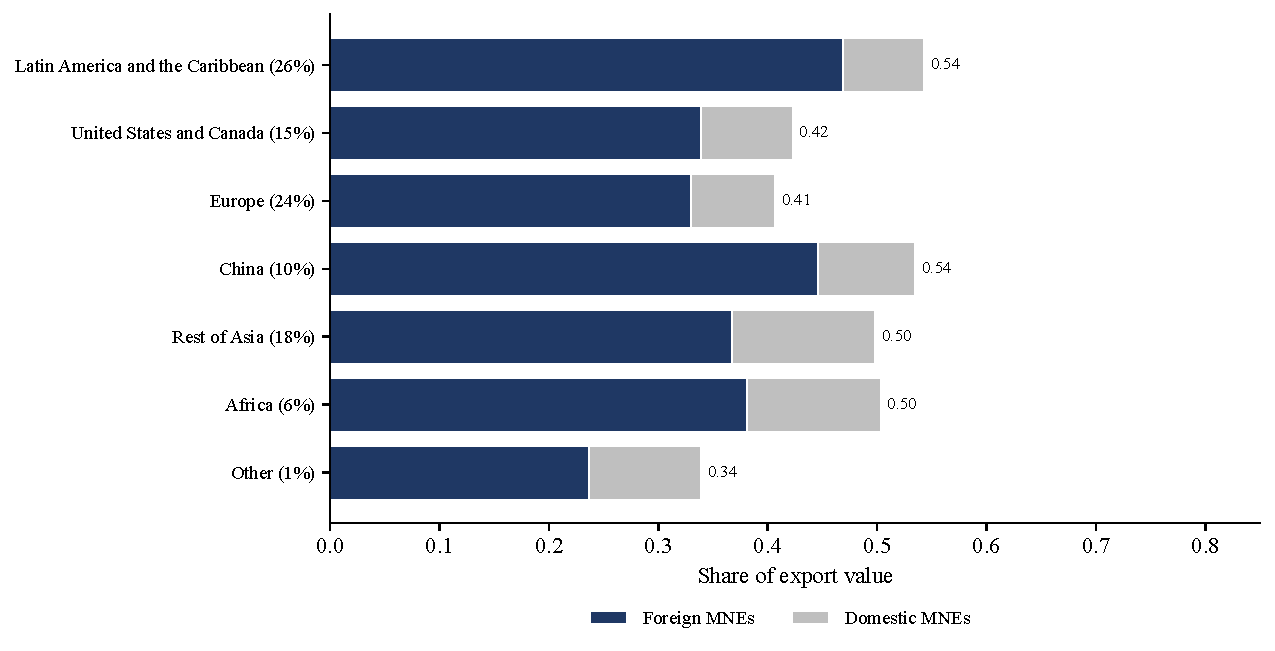
\includegraphics[width=0.85\textwidth,height=0.8\textheight,keepaspectratio]{figures/agro/fig_agp_dest.pdf}%
  \par\vspace{2pt}%
  \parbox{0.92\textwidth}{\footnotesize %
  \textit{Notes:} Shares of the agricultural exports going to each region, by type of exporter, 2012--2018 pooled. In parentheses, the region's share of total agricultural exports.\\[3pt]%
  \srcnote}%
  \end{figure}

\subsection{Ownership by Exporting Country}
% ---- Table: Multinational Share of Agricultural Exports, by Exporting Country
\begin{table}[H]\centering\small%
  \caption{Multinational Share of Agricultural Exports, by Exporting Country}%
  \label{tab:ap_f1n}%
  \adjustbox{max width=\textwidth, max totalheight=0.8\textheight}{\begin{tabular}{lrrrr}
\toprule
Origin & Foreign & Domestic & All MNEs & Value (US\$bn/yr) \\
\midrule
PRY & 0.647 & 0.009 & 0.656 & 6.3 \\
URY & 0.530 & 0.096 & 0.627 & 4.4 \\
CHL & 0.303 & 0.182 & 0.485 & 7.6 \\
ARG & 0.372 & 0.101 & 0.473 & 37.2 \\
CRI & 0.443 & 0.015 & 0.458 & 4.5 \\
DOM & 0.403 & 0.041 & 0.444 & 1.9 \\
COL & 0.282 & 0.148 & 0.430 & 6.9 \\
PER & 0.332 & 0.044 & 0.376 & 8.1 \\
SLV & 0.302 & 0.000 & 0.302 & 1.2 \\
\midrule
All & 0.388 & 0.091 & 0.480 & 78.2 \\
\bottomrule
\end{tabular}
}%
  \par\vspace{3pt}%
  \begin{minipage}{0.95\textwidth}\footnotesize %
  \textit{Notes:} Shares of agricultural export value (HS 01--24), 2012--2018 pooled. Values are annual averages over 2012--2018, in US\$ billion.\\[3pt]%
  \srcnote%
  \end{minipage}%
  \end{table}

% ---- Figure: Multinational Share of Agricultural Exports, by Exporting Country and Parent Country
\begin{figure}[H]\centering%
  \caption{Multinational Share of Agricultural Exports, by Exporting Country and Parent Country}%
  \label{fig:ap_f1_parent}%
  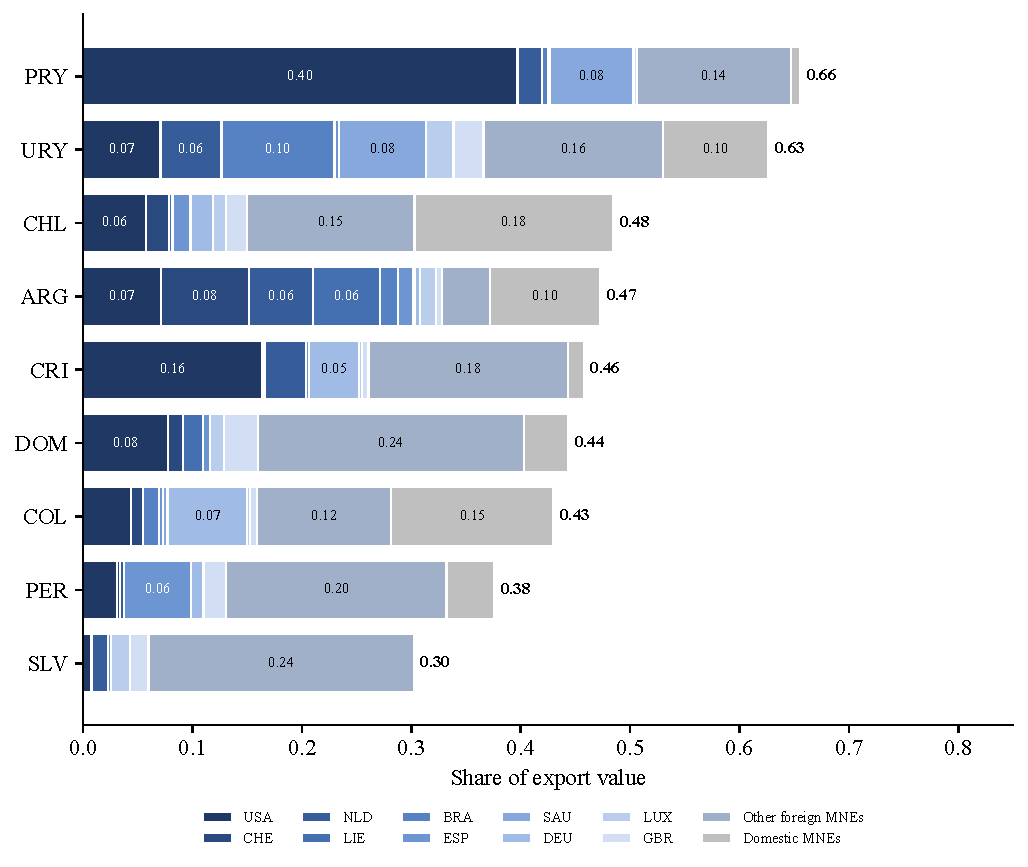
\includegraphics[width=0.92\textwidth,height=0.8\textheight,keepaspectratio]{figures/agro/fig_wp1a_origin_by_parent.pdf}%
  \par\vspace{2pt}%
  \parbox{0.92\textwidth}{\footnotesize %
  \textit{Notes:} Shares of each country's agricultural export value, 2012--2018 pooled. Foreign MNEs split by country of the ultimate parent; the ten largest parent countries are shown separately.\\[3pt]%
  \srcnote}%
  \end{figure}

% ---- Table: Multinational Share of Agricultural Exports, by Exporting Country and Parent Country
\begin{table}[H]\centering\small%
  \caption{Multinational Share of Agricultural Exports, by Exporting Country and Parent Country}%
  \label{tab:ap_f1pn}%
  \adjustbox{max width=\textwidth, max totalheight=0.8\textheight}{\begin{tabular}{lcccccccccccccc}
\toprule
Origin & USA & CHE & NLD & LIE & BRA & ESP & SAU & DEU & LUX & GBR & Other & Domestic & All MNEs & Value (US\$bn/yr) \\
\midrule
PRY & 0.397 & 0.000 & 0.022 & 0.000 & 0.006 & 0.002 & 0.076 & 0.000 & 0.000 & 0.003 & 0.141 & 0.009 & 0.656 & 6.3 \\
URY & 0.071 & 0.000 & 0.055 & 0.001 & 0.103 & 0.004 & 0.080 & 0.000 & 0.025 & 0.028 & 0.164 & 0.096 & 0.627 & 4.4 \\
CHL & 0.057 & 0.021 & 0.000 & 0.003 & 0.001 & 0.016 & 0.000 & 0.021 & 0.012 & 0.019 & 0.153 & 0.182 & 0.485 & 7.6 \\
ARG & 0.071 & 0.080 & 0.059 & 0.061 & 0.016 & 0.014 & 0.002 & 0.004 & 0.014 & 0.006 & 0.044 & 0.101 & 0.473 & 37.2 \\
CRI & 0.164 & 0.002 & 0.038 & 0.000 & 0.000 & 0.003 & 0.000 & 0.046 & 0.003 & 0.006 & 0.182 & 0.015 & 0.458 & 4.5 \\
DOM & 0.078 & 0.014 & 0.000 & 0.018 & 0.000 & 0.006 & 0.000 & 0.000 & 0.013 & 0.031 & 0.243 & 0.041 & 0.444 & 1.9 \\
COL & 0.044 & 0.011 & 0.000 & 0.000 & 0.015 & 0.003 & 0.004 & 0.073 & 0.002 & 0.007 & 0.123 & 0.148 & 0.430 & 6.9 \\
PER & 0.031 & 0.003 & 0.003 & 0.000 & 0.000 & 0.061 & 0.000 & 0.011 & 0.000 & 0.021 & 0.201 & 0.044 & 0.376 & 8.1 \\
SLV & 0.007 & 0.001 & 0.014 & 0.000 & 0.000 & 0.003 & 0.000 & 0.000 & 0.018 & 0.017 & 0.243 & 0.000 & 0.302 & 1.2 \\
\bottomrule
\end{tabular}
}%
  \par\vspace{3pt}%
  \begin{minipage}{0.95\textwidth}\footnotesize %
  \textit{Notes:} Shares of each country's agricultural export value, 2012--2018 pooled. Other: all remaining foreign parents. Values are annual averages over 2012--2018, in US\$ billion.\\[3pt]%
  \srcnote%
  \end{minipage}%
  \end{table}

\subsection{Parent Countries and Destinations}
% ---- Table: Foreign-Multinational Agricultural Exports, by Parent Country: Other Countries and Tax Havens
\begin{table}[H]\centering\small%
  \caption{Foreign-Multinational Agricultural Exports, by Parent Country: Other Countries and Tax Havens}%
  \label{tab:ap_panels}%
  \adjustbox{max width=\textwidth, max totalheight=0.8\textheight}{\begin{tabular}{lrlr}
\toprule
\multicolumn{2}{c}{Panel A. Other parent countries} & \multicolumn{2}{c}{Panel B. Tax havens and conduits} \\
\cmidrule(lr){1-2}\cmidrule(lr){3-4}
Parent country & Share (\%) & Jurisdiction & Share (\%) \\
\midrule
USA & 24.7 & CHE & 11.2 \\
NLD & 9.6 & LIE & 8.1 \\
BRA & 4.1 & LUX & 2.8 \\
ESP & 3.9 & PAN & 2.4 \\
SAU & 3.2 & BMU & 1.7 \\
DEU & 3.2 & HKG & 0.7 \\
GBR & 2.6 & SGP & 0.7 \\
FRA & 2.5 & CYM & 0.3 \\
JPN & 2.3 & MCO & 0.2 \\
JOR & 1.5 & MUS & 0.2 \\
Other & 14.0 & Other & 0.4 \\
\midrule
Total & 71.5 & Total & 28.5 \\
\bottomrule
\end{tabular}
}%
  \par\vspace{3pt}%
  \begin{minipage}{0.95\textwidth}\footnotesize %
  \textit{Notes:} Percent of foreign-MNE agricultural export value with a recorded parent country, by country of the ultimate parent, 2012--2018. The two panels add to 100.\\[3pt]%
  \srcnote%
  \end{minipage}%
  \end{table}

% ---- Table: Foreign-Multinational Agricultural Exports, by Parent Country
\begin{table}[H]\centering\small%
  \caption{Foreign-Multinational Agricultural Exports, by Parent Country}%
  \label{tab:ap_f4n}%
  \adjustbox{max width=\textwidth, max totalheight=0.8\textheight}{\begin{tabular}{lrr}
\toprule
Parent country & Share (\%) & Value (US\$bn/yr) \\
\midrule
USA & 24.7 & 6.6 \\
CHE & 11.2 & 3.0 \\
NLD & 9.6 & 2.6 \\
LIE & 8.1 & 2.2 \\
BRA & 4.1 & 1.1 \\
ESP & 3.9 & 1.0 \\
SAU & 3.2 & 0.9 \\
DEU & 3.2 & 0.9 \\
LUX & 2.8 & 0.7 \\
GBR & 2.6 & 0.7 \\
FRA & 2.5 & 0.7 \\
PAN & 2.4 & 0.6 \\
JPN & 2.3 & 0.6 \\
BMU & 1.7 & 0.5 \\
JOR & 1.5 & 0.4 \\
Other (108 countries) & 16.4 & 4.4 \\
\midrule
All foreign MNEs & 100.0 & 30.4 \\
\bottomrule
\end{tabular}
}%
  \par\vspace{3pt}%
  \begin{minipage}{0.95\textwidth}\footnotesize %
  \textit{Notes:} Percent of foreign-MNE agricultural export value, by country of the ultimate parent, 2012--2018. Values are annual averages over 2012--2018, in US\$ billion.\\[3pt]%
  \srcnote%
  \end{minipage}%
  \end{table}

% ---- Table: Destination of Foreign-Multinational Agricultural Exports, by Parent Country
\begin{table}[H]\centering\small%
  \caption{Destination of Foreign-Multinational Agricultural Exports, by Parent Country}%
  \label{tab:ap_pxd}%
  \adjustbox{max width=\textwidth, max totalheight=0.8\textheight}{\begin{tabular}{lrrrrrrrrrrrr}
\toprule
Top 10 parents / Top 10 destinations & CHN & USA & ARG & BRA & ESP & CHL & URY & NLD & VNM & ITA & Other destinations & Total \\
\midrule
USA & 13.9 & 7.0 & 17.6 & 3.5 & 1.5 & 4.2 & 7.1 & 1.7 & 1.5 & 0.7 & 41.4 & 100.0 \\
CHE & 6.6 & 1.5 & 0.2 & 6.4 & 2.4 & 3.7 & 0.8 & 1.1 & 5.6 & 3.7 & 68.1 & 100.0 \\
NLD & 13.8 & 3.4 & 2.8 & 5.3 & 1.3 & 4.0 & 3.1 & 2.9 & 4.2 & 5.8 & 53.3 & 100.0 \\
LIE & 15.6 & 1.4 & 0.0 & 5.9 & 2.5 & 2.3 & 0.2 & 0.4 & 6.0 & 2.1 & 63.6 & 100.0 \\
BRA & 29.9 & 10.8 & 0.9 & 5.2 & 1.1 & 1.8 & 1.1 & 4.6 & 2.1 & 2.2 & 40.4 & 100.0 \\
ESP & 7.9 & 15.2 & 0.4 & 3.2 & 25.6 & 2.7 & 0.2 & 5.7 & 2.7 & 2.8 & 33.4 & 100.0 \\
SAU & 12.5 & 7.0 & 0.0 & 7.8 & 2.2 & 15.4 & 0.2 & 2.5 & 2.5 & 2.0 & 47.9 & 100.0 \\
DEU & 0.4 & 35.7 & 0.3 & 1.7 & 3.8 & 1.2 & 0.8 & 4.8 & 0.9 & 1.9 & 48.7 & 100.0 \\
LUX & 2.3 & 5.5 & 0.1 & 43.6 & 9.6 & 2.2 & 2.8 & 0.2 & 0.8 & 3.5 & 29.4 & 100.0 \\
GBR & 15.5 & 8.0 & 0.3 & 8.8 & 4.4 & 3.0 & 2.4 & 3.5 & 2.1 & 0.9 & 51.2 & 100.0 \\
Other parents & 7.9 & 22.7 & 8.5 & 8.4 & 3.6 & 1.6 & 2.4 & 3.7 & 0.7 & 1.9 & 38.5 & 100.0 \\
\bottomrule
\end{tabular}
}%
  \par\vspace{3pt}%
  \begin{minipage}{0.95\textwidth}\footnotesize %
  \textit{Notes:} Percent of each parent country's agricultural exports, by destination (rows add to 100), 2012--2018. Ten largest parent countries and ten largest destinations.\\[3pt]%
  \srcnote%
  \end{minipage}%
  \end{table}

% ---- Table: Foreign-Multinational Agricultural Exports to the Parent Countries, by Parent Country
\begin{table}[H]\centering\small%
  \caption{Foreign-Multinational Agricultural Exports to the Parent Countries, by Parent Country}%
  \label{tab:ap_pxp}%
  \adjustbox{max width=\textwidth, max totalheight=0.8\textheight}{\begin{tabular}{lrrrrrrrrrrr}
\toprule
Parent / Destination & USA & CHE & NLD & BRA & ESP & SAU & DEU & LUX & GBR & Other destinations & Total \\
\midrule
USA & 7.0 & 0.0 & 1.7 & 3.5 & 1.5 & 0.9 & 0.5 & 0.0 & 0.4 & 84.5 & 100.0 \\
CHE & 1.5 & 0.0 & 1.1 & 6.4 & 2.4 & 3.8 & 0.4 & 0.0 & 0.8 & 83.7 & 100.0 \\
NLD & 3.4 & 0.0 & 2.9 & 5.3 & 1.3 & 1.0 & 0.6 & 0.0 & 0.9 & 84.4 & 100.0 \\
LIE & 1.4 & 0.0 & 0.4 & 5.9 & 2.5 & 3.6 & 0.1 & 0.0 & 0.5 & 85.6 & 100.0 \\
BRA & 10.8 & 0.5 & 4.6 & 5.2 & 1.1 & 1.0 & 5.3 & 0.0 & 0.9 & 70.6 & 100.0 \\
ESP & 15.2 & 0.0 & 5.7 & 3.2 & 25.6 & 0.4 & 1.5 & 0.0 & 1.9 & 46.4 & 100.0 \\
SAU & 7.0 & 0.7 & 2.5 & 7.8 & 2.2 & 2.8 & 1.1 & 0.0 & 1.5 & 74.4 & 100.0 \\
DEU & 35.7 & 0.1 & 4.8 & 1.7 & 3.8 & 0.3 & 7.2 & 0.0 & 1.0 & 45.5 & 100.0 \\
LUX & 5.5 & 0.1 & 0.2 & 43.6 & 9.6 & 0.0 & 0.2 & 0.0 & 0.4 & 40.4 & 100.0 \\
GBR & 8.0 & 0.2 & 3.5 & 8.8 & 4.4 & 0.0 & 2.3 & 0.0 & 1.6 & 71.3 & 100.0 \\
Other parents & 22.7 & 0.4 & 3.7 & 8.4 & 3.6 & 0.3 & 1.9 & 0.0 & 2.0 & 56.9 & 100.0 \\
\bottomrule
\end{tabular}
}%
  \par\vspace{3pt}%
  \begin{minipage}{0.95\textwidth}\footnotesize %
  \textit{Notes:} Percent of each parent country's agricultural exports, by destination (rows add to 100), 2012--2018. Destinations are the ten largest parent countries; the diagonal is the share shipped to the parent's own country.\\[3pt]%
  \srcnote%
  \end{minipage}%
  \end{table}

% ---- Table: Destination of Multinational Agricultural Exports, by Parent Region
\begin{table}[H]\centering\small%
  \caption{Destination of Multinational Agricultural Exports, by Parent Region}%
  \label{tab:ap_reg}%
  \adjustbox{max width=\textwidth, max totalheight=0.8\textheight}{\begin{tabular}{lrrrrrrrr}
\toprule
Parent region / Destination region & Latin America & North America & Europe & Asia & Africa & Oceania & Rest of World & Total \\
\midrule
Latin America & 29.9 & 16.4 & 20.2 & 30.0 & 3.1 & 0.3 & 0.1 & 100.0 \\
North America & 50.2 & 7.6 & 10.7 & 24.2 & 7.2 & 0.1 & 0.0 & 100.0 \\
Europe & 27.4 & 9.2 & 21.7 & 32.9 & 8.2 & 0.6 & 0.0 & 100.0 \\
Asia & 14.5 & 30.5 & 24.9 & 27.3 & 2.4 & 0.3 & 0.1 & 100.0 \\
Africa & 29.8 & 14.6 & 32.9 & 11.8 & 8.6 & 0.3 & 1.9 & 100.0 \\
Oceania & 59.9 & 17.8 & 9.1 & 7.2 & 0.6 & 5.3 & 0.0 & 100.0 \\
Rest of World & 18.5 & 35.7 & 26.1 & 18.9 & 0.0 & 0.8 & 0.0 & 100.0 \\
Domestic MNEs & 21.5 & 13.6 & 19.8 & 35.5 & 8.4 & 1.1 & 0.1 & 100.0 \\
Local firms & 23.3 & 16.5 & 26.9 & 26.1 & 6.0 & 1.2 & 0.1 & 100.0 \\
\bottomrule
\end{tabular}
}%
  \par\vspace{3pt}%
  \begin{minipage}{0.95\textwidth}\footnotesize %
  \textit{Notes:} Percent of each group's agricultural exports, by destination region (rows add to 100), 2012--2018. Domestic MNEs and local firms are shown for comparison.\\[3pt]%
  \srcnote%
  \end{minipage}%
  \end{table}

% ---- Figure: Destination of Foreign-Multinational Agricultural Exports: Fifteen Largest Parent Countries and Destinations
\begin{figure}[H]\centering%
  \caption{Destination of Foreign-Multinational Agricultural Exports: Fifteen Largest Parent Countries and Destinations}%
  \label{fig:ap_hm}%
  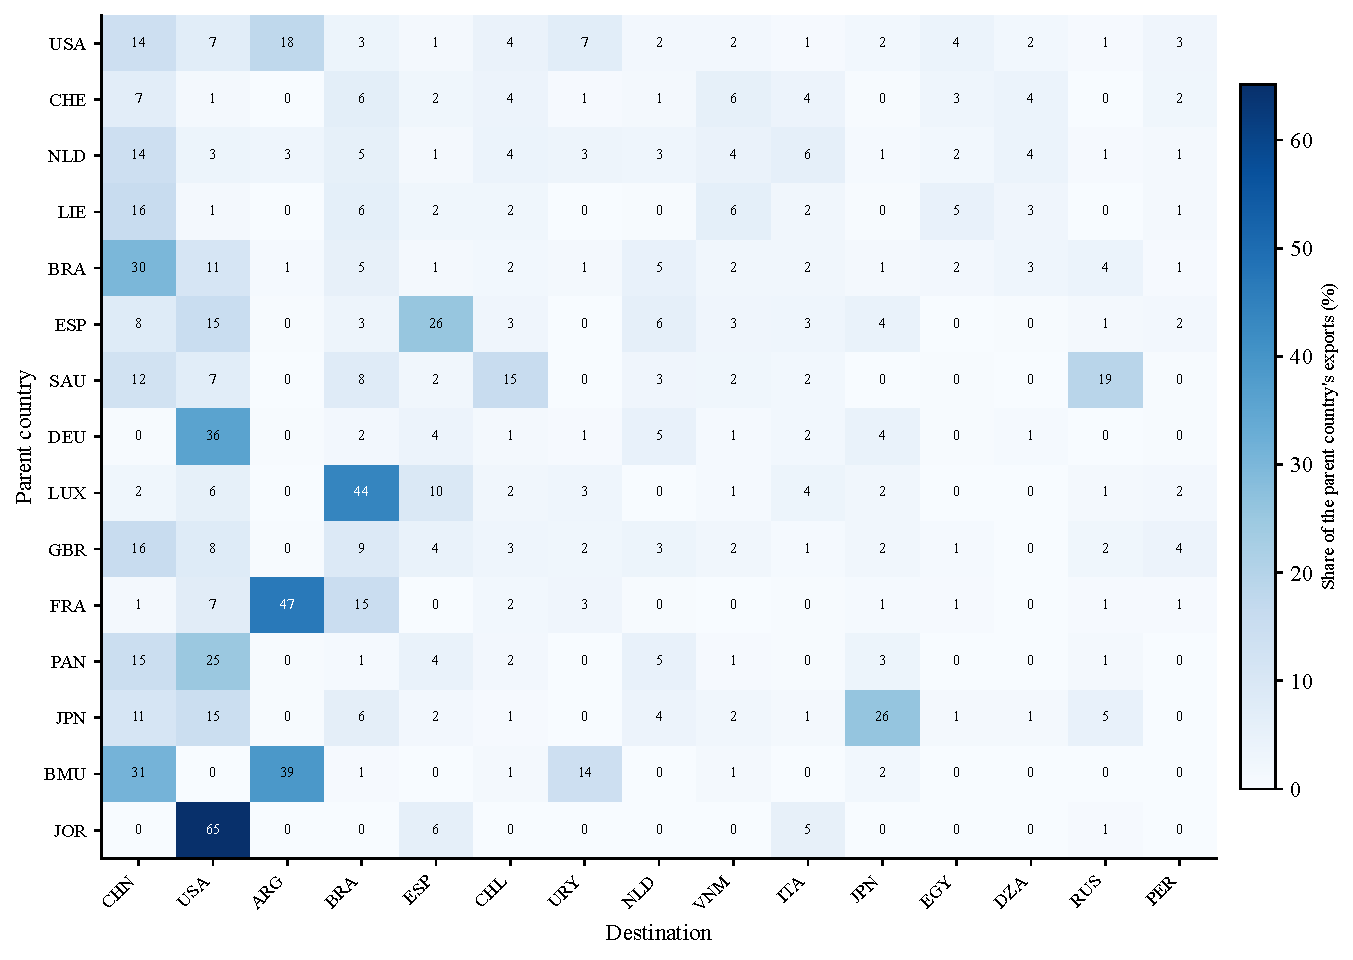
\includegraphics[width=1.0\textwidth,height=0.8\textheight,keepaspectratio]{figures/agro/fig_wp1d_heatmap_country_rowpct.pdf}%
  \par\vspace{2pt}%
  \parbox{0.92\textwidth}{\footnotesize %
  \textit{Notes:} Percent of each parent country's agricultural exports going to each destination, 2012--2018 (rows add to 100 including other destinations).\\[3pt]%
  \srcnote}%
  \end{figure}

% ---- Figure: Share of Foreign-Multinational Agricultural Exports Shipped to the Parent Country
\begin{figure}[H]\centering%
  \caption{Share of Foreign-Multinational Agricultural Exports Shipped to the Parent Country}%
  \label{fig:ap_home}%
  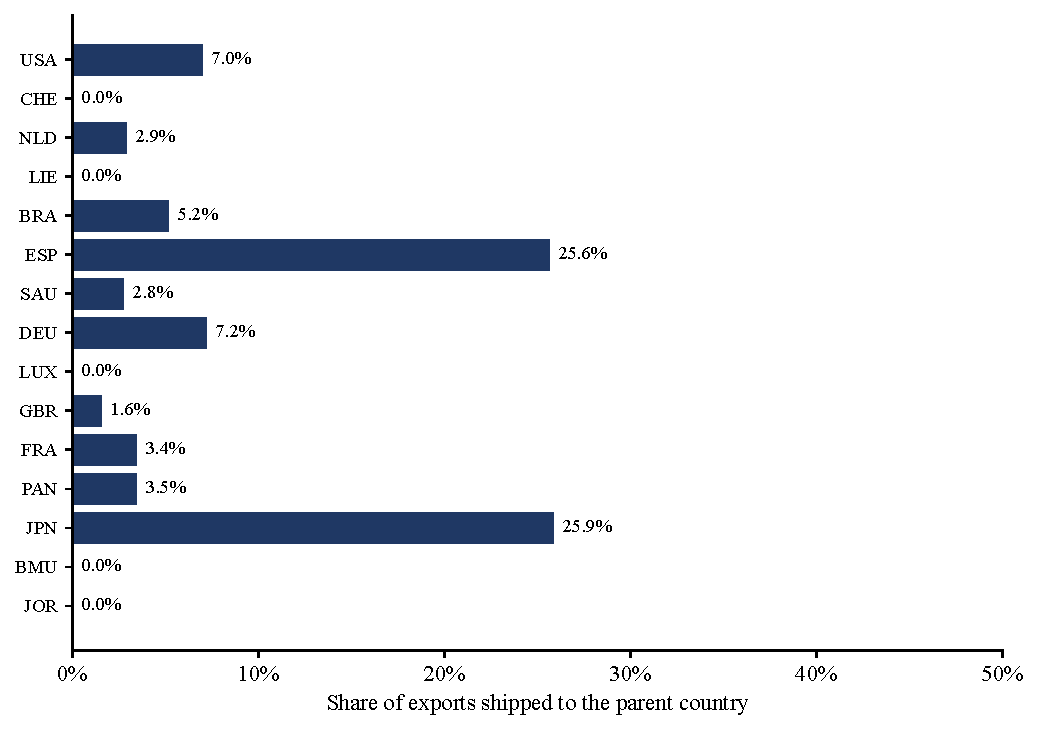
\includegraphics[width=0.85\textwidth,height=0.8\textheight,keepaspectratio]{figures/agro/fig_wp1d_home_share_by_parent.pdf}%
  \par\vspace{2pt}%
  \parbox{0.92\textwidth}{\footnotesize %
  \textit{Notes:} Percent of each parent country's agricultural exports shipped to that same country, 2012--2018.\\[3pt]%
  \srcnote}%
  \end{figure}

\subsection{Multinational Groups}
% ---- Table: Foreign-Multinational Agricultural Exports and Number of Parents, by Size of the Group's Global Network
\begin{table}[H]\centering\small%
  \caption{Foreign-Multinational Agricultural Exports and Number of Parents, by Size of the Group's Global Network}%
  \label{tab:ap_f5_tab}%
  \adjustbox{max width=\textwidth, max totalheight=0.8\textheight}{\begin{tabular}{lrrr}
\toprule
Affiliates worldwide & Parents & Share of parents (\%) & Share of foreign-MNE export value (\%) \\
\midrule
1 & 1,128 & 43.9 & 8.7 \\
2--10 & 727 & 28.3 & 11.0 \\
11--100 & 383 & 14.9 & 29.8 \\
$>$100 & 334 & 13.0 & 50.6 \\
\midrule
All parents & 2,572 & 100 & 100 \\
\bottomrule
\end{tabular}
}%
  \par\vspace{3pt}%
  \begin{minipage}{0.95\textwidth}\footnotesize %
  \textit{Notes:} Number and share of parents, and share of foreign-MNE agricultural export value, by the number of affiliates the group has worldwide, 2012--2018.\\[3pt]%
  \srcnote%
  \end{minipage}%
  \end{table}

\subsection{Multinational Presence: Additional Results}
% ---- Table: Multinational Presence and Agricultural Exports: Extensive Margin, by Type of Multinational
\begin{table}[H]\centering\small%
  \caption{Multinational Presence and Agricultural Exports: Extensive Margin, by Type of Multinational}%
  \label{tab:ap_ext}%
  \adjustbox{max width=\textwidth, max totalheight=0.8\textheight}{\begin{tabular}{lcccccc} \hline
 & \multicolumn{2}{c}{All MNEs} & \multicolumn{2}{c}{Foreign / domestic} & \multicolumn{2}{c}{Foreign by destination, domestic} \\
 & (1) & (2) & (3) & (4) & (5) & (6) \\ \hline
\multicolumn{7}{l}{\textit{Panel A. Dependent variable: $\ln$ exports, all firms}} \\
Any MNE present & 1.8195*** & 0.6549*** &  &  &  &  \\
 & (0.0647) & (0.0262) &  &  &  &  \\
Any foreign MNE &  &  & 1.8339*** & 0.6562*** &  &  \\
 &  &  & (0.0601) & (0.0241) &  &  \\
Any foreign MNE, parent-country destination &  &  &  &  & 1.7064*** & 0.5045*** \\
 &  &  &  &  & (0.1231) & (0.0762) \\
Any foreign MNE, other destination &  &  &  &  & 1.8214*** & 0.6550*** \\
 &  &  &  &  & (0.0599) & (0.0243) \\
Any domestic MNE &  &  & 1.6332*** & 0.5286*** & 1.5796*** & 0.5251*** \\
 &  &  & (0.0626) & (0.0264) & (0.0607) & (0.0263) \\
\midrule
\multicolumn{7}{l}{\textit{Panel B. Dependent variable: $\ln$ exports, non-MNE firms}} \\
Any MNE present & 1.9479*** & 0.2390*** &  &  &  &  \\
 & (0.0628) & (0.0210) &  &  &  &  \\
Any foreign MNE &  &  & 1.7962*** & 0.2527*** &  &  \\
 &  &  & (0.0629) & (0.0212) &  &  \\
Any foreign MNE, parent-country destination &  &  &  &  & 1.4837*** & 0.2394*** \\
 &  &  &  &  & (0.1096) & (0.0500) \\
Any foreign MNE, other destination &  &  &  &  & 1.7648*** & 0.2555*** \\
 &  &  &  &  & (0.0623) & (0.0210) \\
Any domestic MNE &  &  & 1.3273*** & 0.2076*** & 1.2707*** & 0.2058*** \\
 &  &  & (0.0562) & (0.0221) & (0.0526) & (0.0219) \\
\hline
Product FE & $\checkmark$ &  & $\checkmark$ &  & $\checkmark$ &  \\
Origin $\times$ year FE & $\checkmark$ &  & $\checkmark$ &  & $\checkmark$ &  \\
Destination $\times$ year FE & $\checkmark$ &  & $\checkmark$ &  & $\checkmark$ &  \\
Origin $\times$ dest.\ $\times$ product FE &  & $\checkmark$ &  & $\checkmark$ &  & $\checkmark$ \\
Origin $\times$ dest.\ $\times$ year FE &  & $\checkmark$ &  & $\checkmark$ &  & $\checkmark$ \\
Observations (Panel A) & 198,142 & 175,847 & 198,142 & 175,847 & 198,142 & 175,847 \\
Observations (Panel B) & 156,915 & 137,240 & 156,915 & 137,240 & 156,915 & 137,240 \\
\hline
\end{tabular}
}%
  \par\vspace{3pt}%
  \begin{minipage}{0.95\textwidth}\footnotesize %
  \textit{Notes:} Regression at the origin country, destination country, product and year level; agricultural products, 2012--2018. Dependent variable: $\ln$ exports (Panel A) and $\ln$ exports of local firms (Panel B). Regressors: indicators for at least one MNE of each type. Columns (5)--(6) split foreign MNEs by whether the destination is the parent's country. Standard errors clustered by origin--destination pair in parentheses. *** $p<0.01$, ** $p<0.05$, * $p<0.1$.\\[3pt]%
  \srcnote%
  \end{minipage}%
  \end{table}

% ---- Table: Multinational Agricultural Exports by Exporting Country and Destination Type
\begin{table}[H]\centering\small%
  \caption{Multinational Agricultural Exports by Exporting Country and Destination Type}%
  \label{tab:ap_pres}%
  \adjustbox{max width=\textwidth, max totalheight=0.8\textheight}{\begin{tabular}{lrrrrr}
\toprule
Origin & MNE value (US\$bn/yr) & of which domestic (\%) & Foreign-MNE value (US\$bn/yr) & \multicolumn{2}{c}{\% of foreign-MNE value, by destination} \\
 & & & & parent country & other (of which: group affiliate there) \\
\midrule
ARG & 17.6 & 21.3 & 13.9 & 2.9 & 97.1 (29.6) \\
CHL & 3.7 & 37.5 & 2.3 & 11.3 & 88.7 (30.2) \\
COL & 3.0 & 34.5 & 2.0 & 4.7 & 95.3 (32.5) \\
CRI & 2.0 & 3.2 & 2.0 & 10.1 & 89.9 (45.9) \\
DOM & 0.9 & 9.2 & 0.8 & 13.7 & 86.3 (9.7) \\
PER & 3.0 & 11.6 & 2.7 & 4.5 & 95.5 (14.9) \\
PRY & 4.2 & 1.3 & 4.1 & 1.9 & 98.1 (70.0) \\
SLV & 0.4 & 0.0 & 0.4 & 12.1 & 87.9 (59.3) \\
URY & 2.8 & 15.4 & 2.4 & 3.0 & 97.0 (42.7) \\
\midrule
All & 37.5 & 19.1 & 30.4 & 4.5 & 95.5 (35.9) \\
\bottomrule
\end{tabular}
}%
  \par\vspace{3pt}%
  \begin{minipage}{0.95\textwidth}\footnotesize %
  \textit{Notes:} MNE and foreign-MNE agricultural export value by country, and the split of foreign-MNE value by destination, 2012--2018. Parent country: exports to the country of the ultimate parent. Other: all remaining destinations; in parentheses, destinations where the group has another affiliate. Values are annual averages over 2012--2018, in US\$ billion.\\[3pt]%
  \srcnote%
  \end{minipage}%
  \end{table}

\subsection{Product Groups}
% ---- Figure: Multinational Share of Agricultural Exports, by Product Group
\begin{figure}[H]\centering%
  \caption{Multinational Share of Agricultural Exports, by Product Group}%
  \label{fig:ap_sitc}%
  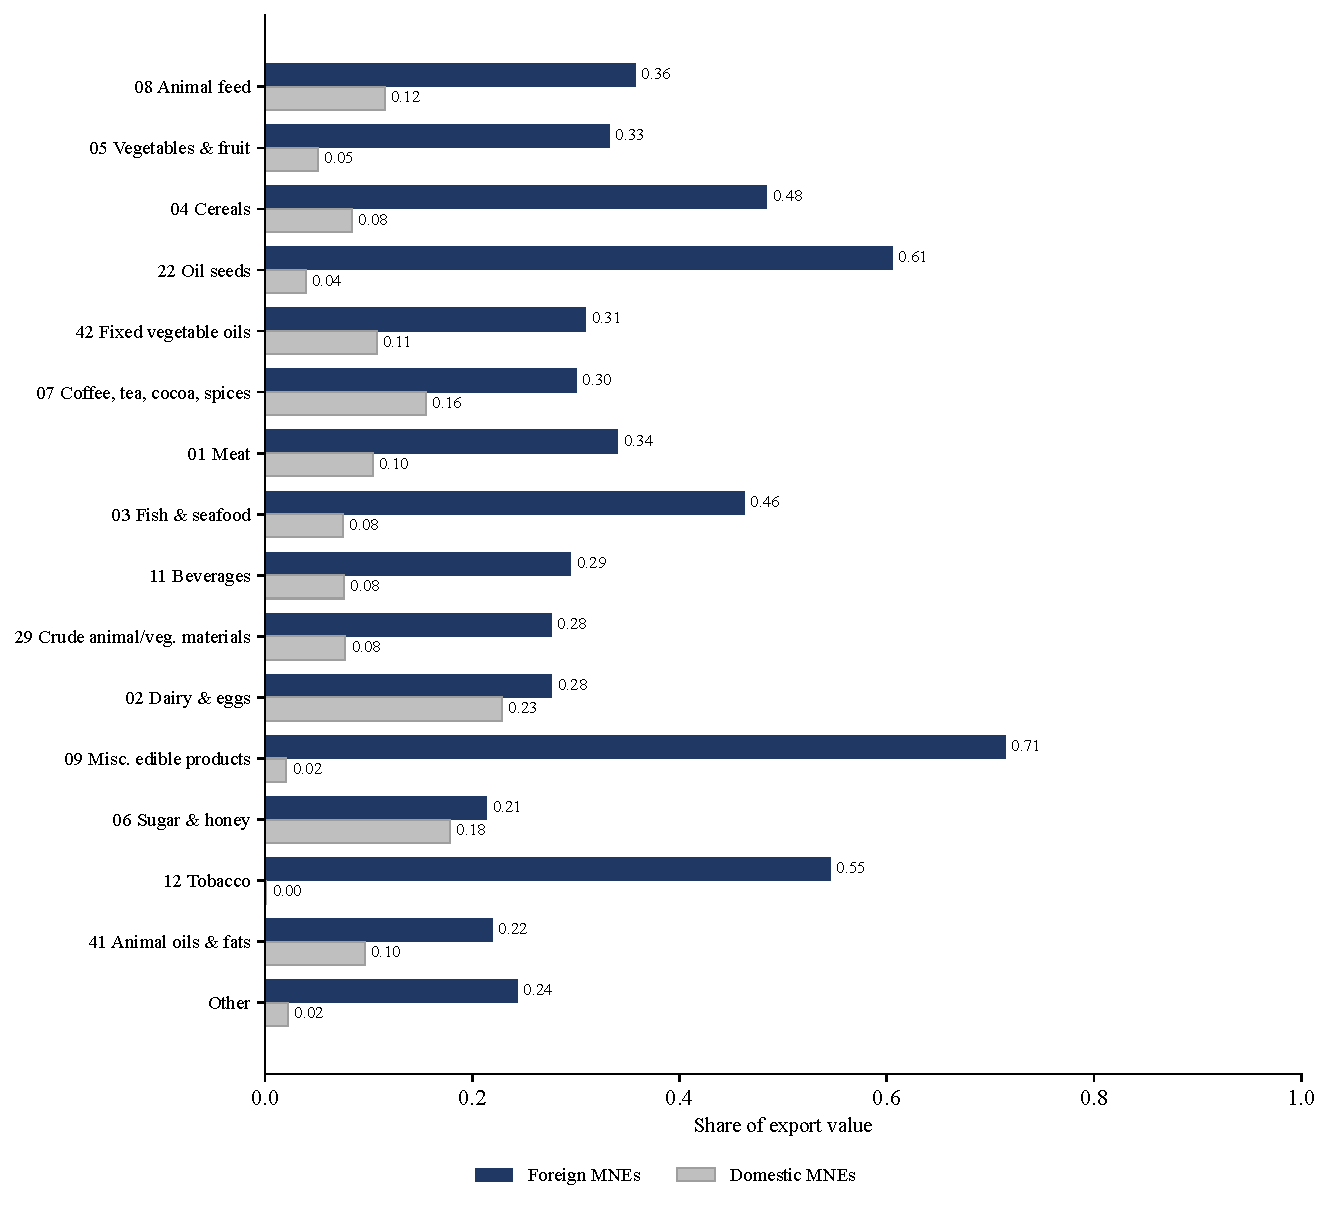
\includegraphics[width=0.9\textwidth,height=0.8\textheight,keepaspectratio]{figures/agro/fig_wp2_sitc2.pdf}%
  \par\vspace{2pt}%
  \parbox{0.92\textwidth}{\footnotesize %
  \textit{Notes:} Shares of each SITC Rev.\,3 division's export value, 2012--2018 pooled. Divisions ordered by export value.\\[3pt]%
  \srcnote}%
  \end{figure}

% ---- Table: Agricultural Exports and Multinational Shares: Inputs and Other Products
\begin{table}[H]\centering\footnotesize%
  \caption{Agricultural Exports and Multinational Shares: Inputs and Other Products}%
  \label{tab:ap_inputs}%
  \adjustbox{max width=\textwidth, max totalheight=0.8\textheight}{\begin{tabular}{@{}l r r r r l@{}}
\toprule
Inputs vs output & Total exports (US\$bn/yr) & MNE exports (US\$bn/yr) & Foreign (\%) & Domestic (\%) & Leading parents (share of foreign) \\
\midrule
Agricultural inputs & 15.1 & 7.1 & 36.0 & 10.9 & CHE 0.26, USA 0.18, LIE 0.18 \\
Agricultural output (food, fibres, beverages) & 63.1 & 30.4 & 39.5 & 8.7 & USA 0.26, NLD 0.09, CHE 0.08 \\
\midrule
All & 78.2 & 37.5 & 38.8 & 9.1 & \\
\bottomrule
\end{tabular}
}%
  \par\vspace{3pt}%
  \begin{minipage}{0.95\textwidth}\footnotesize %
  \textit{Notes:} Inputs: seeds, animal feed and live animals. Foreign and domestic: percent of the group's export value, 2012--2018. Leading parents: the three largest parent countries and their share of the group's foreign-MNE exports. Values are annual averages over 2012--2018, in US\$ billion.\\[3pt]%
  \srcnote%
  \end{minipage}%
  \end{table}

% ---- Figure: Multinational Share of Agricultural Exports: Inputs and Other Products
\begin{figure}[H]\centering%
  \caption{Multinational Share of Agricultural Exports: Inputs and Other Products}%
  \label{fig:ap_inputs}%
  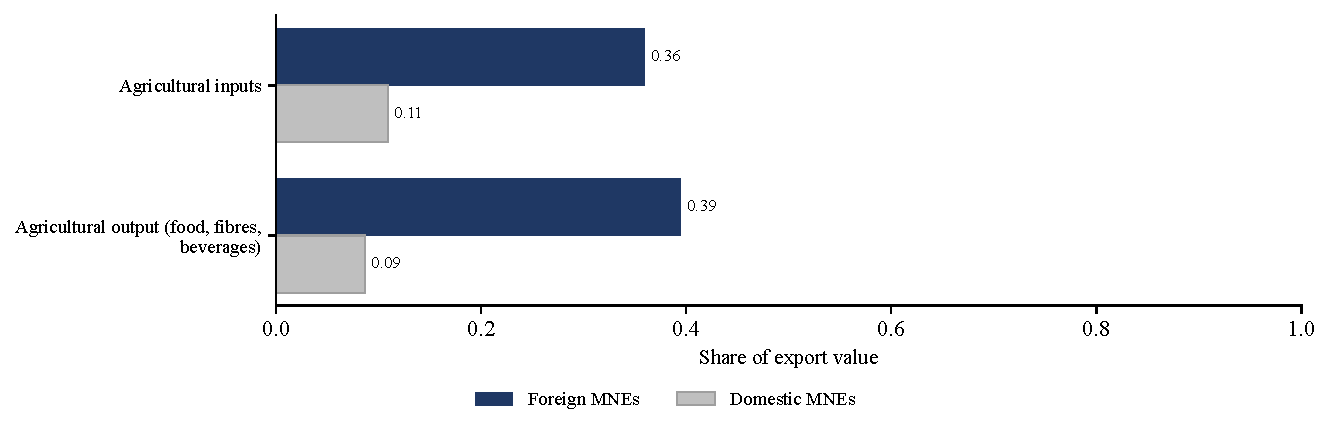
\includegraphics[width=0.7\textwidth,height=0.8\textheight,keepaspectratio]{figures/agro/fig_wp2_inputs.pdf}%
  \par\vspace{2pt}%
  \parbox{0.92\textwidth}{\footnotesize %
  \textit{Notes:} Shares of export value, 2012--2018 pooled. Inputs: seeds, animal feed and live animals.\\[3pt]%
  \srcnote}%
  \end{figure}

% ---- Table: Largest Agricultural Input Products
\begin{table}[H]\centering\footnotesize%
  \caption{Largest Agricultural Input Products}%
  \label{tab:ap_topinputs}%
  \adjustbox{max width=\textwidth, max totalheight=0.8\textheight}{\begin{tabular}{@{}l p{7.5cm} r r r@{}}
\toprule
Product code & Description & US\$bn/yr & Foreign (\%) & Domestic (\%) \\
\midrule
230400 & Oil-cake \& other solid residues, whether/not ground/in pellets, from extraction of soyabean oil & 11.06 & 35 & 12 \\
230120 & Flours, meals \& pellets of fish/of crustaceans, molluscs/other aquatic invertebrates & 1.62 & 31 & 11 \\
230990 & Preparations of a kind used in animal feeding other than dog/cat food put up for RS & 0.56 & 58 & 3 \\
071333 & Kidney beans, incl. white pea beans (Phaseolus vulgaris), dried, shelled, whether/not skinned/split & 0.29 & 27 & 4 \\
230250 & Bran, sharps \& other residues, whether/not in the form of pellets, derived from the sifting/milling/other working of leguminous plants & 0.28 & 29 & 16 \\
100510 & Maize (corn), seed & 0.22 & 61 & 3 \\
230910 & Dog/cat food, put up for RS & 0.19 & 83 & 5 \\
120991 & Vegetable seeds, of a kind used for sowing & 0.12 & 69 & 1 \\
230630 & Oil-cake \& other solid residues, whether/not ground/in pellets, from extraction of sunflower seeds & 0.12 & 22 & 2 \\
071320 & Chickpeas (garbanzos), dried, shelled, whether/not skinned/split & 0.09 & 23 & 2 \\
230800 & Vegetable materials/waste/residues/by-products, whether/not in pellets, of a kind used in animal feeding, n.e.s. & 0.08 & 19 & 0 \\
010290 & Live bovine animals other than pure-bred breeding animals & 0.06 & 33 & 0 \\
100610 & Rice in the husk (paddy/rough) & 0.06 & 46 & 7 \\
230110 & Flours, meals \& pellets of meat/meat offal; greaves & 0.06 & 28 & 0 \\
051199 & Animal products not elsewhere specified/incld. (excl. of 0511.10); dead animals of Ch. 1, unfit for human consumption & 0.04 & 43 & 5 \\
071310 & Peas (Pisum sativum), dried, shelled, whether/not skinned/split & 0.03 & 20 & 1 \\
230230 & Bran, sharps \& other residues, whether/not in the form of pellets, derived from the sifting/milling/other working of wheat & 0.02 & 14 & 1 \\
071339 & Beans (Vigna spp., Phaseolus spp. (excl. of 0713.31-0713.33)), dried, shelled, whether/not skinned/split & 0.02 & 13 & 2 \\
010511 & Live fowls of species Gallus domesticus, weighing not >185g & 0.02 & 3 & 0 \\
071331 & Beans of the species Vigna mungo (L.)/Hepper/Vigna radiata (L.) Wilczek, dried, shelled, whether/not skinned/split & 0.02 & 24 & 1 \\
\bottomrule
\end{tabular}
}%
  \par\vspace{3pt}%
  \begin{minipage}{0.95\textwidth}\footnotesize %
  \textit{Notes:} Input products with the largest export value, 2012--2018. Foreign and domestic: percent of the product's export value. Values are annual averages over 2012--2018, in US\$ billion.\\[3pt]%
  \srcnote%
  \end{minipage}%
  \end{table}

% ---- Table: Agricultural Exports and Multinational Shares, by HS Section
\begin{table}[H]\centering\footnotesize%
  \caption{Agricultural Exports and Multinational Shares, by HS Section}%
  \label{tab:ap_hssection}%
  \adjustbox{max width=\textwidth, max totalheight=0.8\textheight}{\begin{tabular}{@{}l r r r r l@{}}
\toprule
HS section & Total exports (US\$bn/yr) & MNE exports (US\$bn/yr) & Foreign (\%) & Domestic (\%) & Leading parents (share of foreign) \\
\midrule
I Live animals; animal products & 12.0 & 5.8 & 34.8 & 13.3 & SAU 0.19, ESP 0.12, JPN 0.11 \\
II Vegetable products & 32.9 & 16.3 & 42.6 & 6.9 & USA 0.34, NLD 0.11, LIE 0.08 \\
III Fats and oils & 6.7 & 2.8 & 31.6 & 10.2 & CHE 0.26, NLD 0.22, USA 0.21 \\
IV Prepared foodstuffs, beverages, tobacco & 26.6 & 12.7 & 37.8 & 9.8 & USA 0.21, CHE 0.17, LIE 0.10 \\
\midrule
All & 78.2 & 37.5 & 38.8 & 9.1 & \\
\bottomrule
\end{tabular}
}%
  \par\vspace{3pt}%
  \begin{minipage}{0.95\textwidth}\footnotesize %
  \textit{Notes:} Foreign and domestic: percent of the section's export value, 2012--2018. Leading parents: the three largest parent countries and their share of the section's foreign-MNE exports. Values are annual averages over 2012--2018, in US\$ billion.\\[3pt]%
  \srcnote%
  \end{minipage}%
  \end{table}

% ---- Figure: Multinational Share of Agricultural Exports, by HS Section
\begin{figure}[H]\centering%
  \caption{Multinational Share of Agricultural Exports, by HS Section}%
  \label{fig:ap_hssection}%
  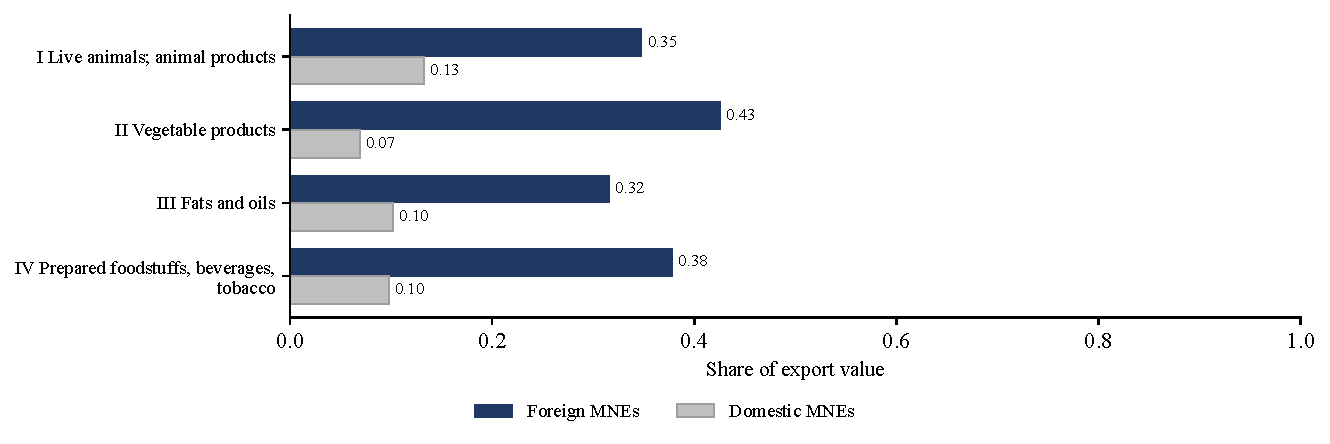
\includegraphics[width=0.9\textwidth,height=0.8\textheight,keepaspectratio]{figures/agro/fig_wp2_hs_section.pdf}%
  \par\vspace{2pt}%
  \parbox{0.92\textwidth}{\footnotesize %
  \textit{Notes:} Shares of each section's export value, 2012--2018 pooled.\\[3pt]%
  \srcnote}%
  \end{figure}

% ---- Table: Agricultural Exports and Multinational Shares, by End Use
\begin{table}[H]\centering\footnotesize%
  \caption{Agricultural Exports and Multinational Shares, by End Use}%
  \label{tab:ap_bec}%
  \adjustbox{max width=\textwidth, max totalheight=0.8\textheight}{\begin{tabular}{@{}l r r r r l@{}}
\toprule
BEC end use & Total exports (US\$bn/yr) & MNE exports (US\$bn/yr) & Foreign (\%) & Domestic (\%) & Leading parents (share of foreign) \\
\midrule
Intermediate & 42.5 & 21.5 & 41.5 & 9.0 & USA 0.31, CHE 0.16, NLD 0.13 \\
Consumption & 29.6 & 13.4 & 36.2 & 9.1 & USA 0.16, ESP 0.10, SAU 0.08 \\
Capital & 0.0 & 0.0 & 17.3 & 1.6 & SAU 0.41, GBR 0.30, NLD 0.27 \\
\midrule
All & 72.2 & 34.9 & 39.3 & 9.0 & \\
\bottomrule
\end{tabular}
}%
  \par\vspace{3pt}%
  \begin{minipage}{0.95\textwidth}\footnotesize %
  \textit{Notes:} End use from BEC Rev.\,4, 2012--2018. Foreign and domestic: percent of the category's export value. Leading parents: the three largest parent countries and their share of the category's foreign-MNE exports. Values are annual averages over 2012--2018, in US\$ billion.\\[3pt]%
  \srcnote%
  \end{minipage}%
  \end{table}

% ---- Figure: Ownership of the Twenty Largest Agricultural Export Products, by Parent Country
\begin{figure}[H]\centering%
  \caption{Ownership of the Twenty Largest Agricultural Export Products, by Parent Country}%
  \label{fig:ap_hs6_parent}%
  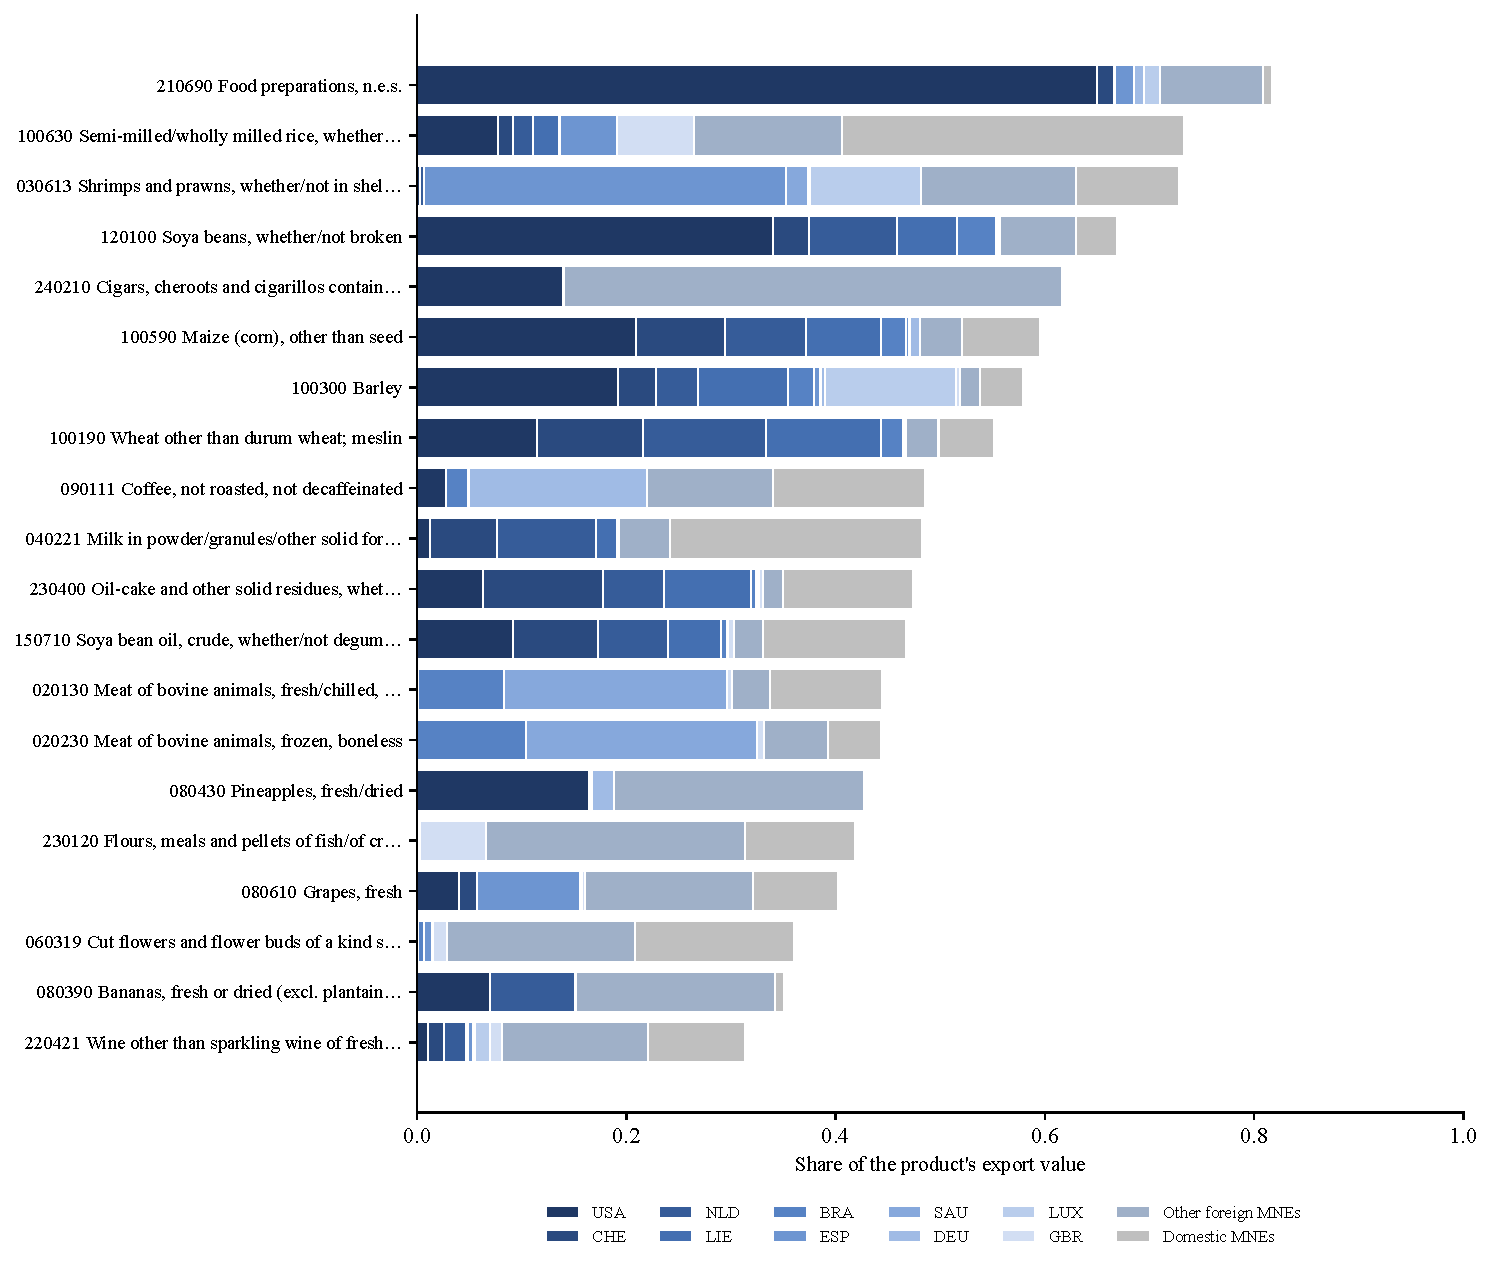
\includegraphics[width=1.0\textwidth,height=0.8\textheight,keepaspectratio]{figures/agro/fig_wp1f_top20_hs6_by_parent.pdf}%
  \par\vspace{2pt}%
  \parbox{0.92\textwidth}{\footnotesize %
  \textit{Notes:} Shares of each product's export value, 2012--2018. Foreign-MNE share split by country of the ultimate parent; the unfilled part of each bar is local firms.\\[3pt]%
  \srcnote}%
  \end{figure}

% ---- Figure: Foreign-Multinational Share of Agricultural Exports, by Exporting Country and Product Group
\begin{figure}[H]\centering%
  \caption{Foreign-Multinational Share of Agricultural Exports, by Exporting Country and Product Group}%
  \label{fig:ap_oxs}%
  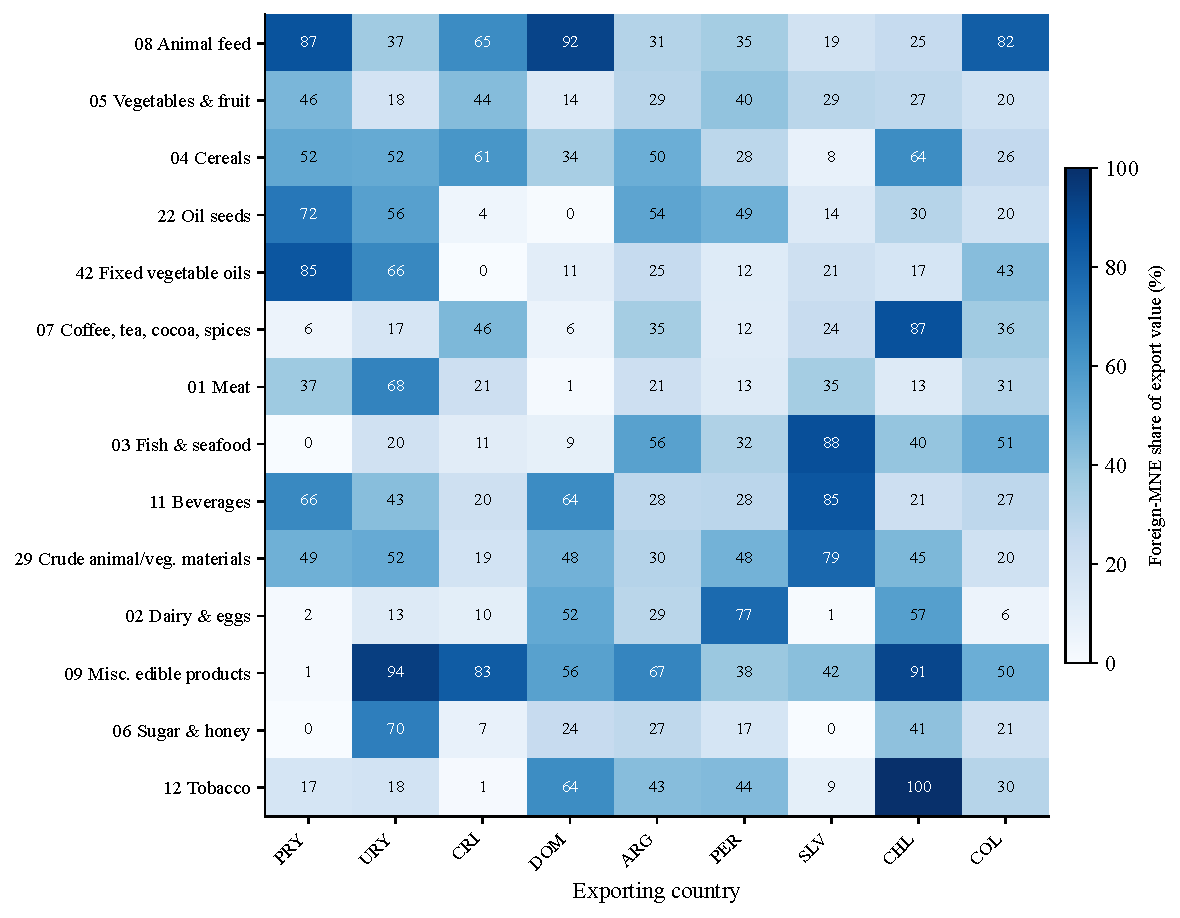
\includegraphics[width=1.0\textwidth,height=0.8\textheight,keepaspectratio]{figures/agro/fig_wp2_origin_x_sitc2.pdf}%
  \par\vspace{2pt}%
  \parbox{0.92\textwidth}{\footnotesize %
  \textit{Notes:} Percent of each SITC division's export value in each country shipped by foreign MNEs, 2012--2018.\\[3pt]%
  \srcnote}%
  \end{figure}

% ---- Table: Agricultural Exports and Foreign-Multinational Shares, by Exporting Country and Product Group
\begin{table}[H]\centering\footnotesize%
  \caption{Agricultural Exports and Foreign-Multinational Shares, by Exporting Country and Product Group}%
  \label{tab:ap_oxs_tab}%
  \adjustbox{max width=\textwidth, max totalheight=0.8\textheight}{\begin{tabular}{lrrrrrrrrrr}
\toprule
SITC division & ARG & CHL & COL & CRI & DOM & PER & PRY & SLV & URY & All \\
\midrule
\multicolumn{11}{l}{\textit{Panel A: composition of the origin's exports, \% (columns sum to 100)}} \\
08 Animal feed & 29.6 & 4.4 & 0.7 & 1.7 & 0.7 & 19.7 & 16.7 & 2.3 & 1.1 & 19.5 \\
05 Vegetables \& fruit & 7.6 & 46.6 & 3.1 & 46.2 & 20.6 & 37.6 & 0.3 & 7.6 & 1.8 & 14.5 \\
04 Cereals & 20.7 & 3.3 & 2.5 & 3.9 & 5.5 & 3.5 & 12.2 & 22.8 & 22.0 & 14.3 \\
22 Oil seeds & 9.9 & 0.4 & 0.0 & 0.0 & 0.0 & 0.3 & 39.3 & 0.0 & 24.6 & 9.8 \\
42 Fixed vegetable oils & 12.3 & 0.6 & 6.2 & 5.4 & 1.2 & 0.6 & 9.1 & 0.3 & 0.1 & 8.0 \\
07 Coffee, tea, cocoa, spices & 0.9 & 0.7 & 46.6 & 10.4 & 11.4 & 13.5 & 0.1 & 18.5 & 0.3 & 6.8 \\
01 Meat & 5.2 & 8.3 & 1.4 & 3.0 & 0.7 & 0.2 & 18.1 & 1.4 & 26.3 & 6.5 \\
03 Fish \& seafood & 4.4 & 5.0 & 1.6 & 1.4 & 0.6 & 12.9 & 0.0 & 10.5 & 2.4 & 4.5 \\
11 Beverages & 2.5 & 18.3 & 0.5 & 1.9 & 6.9 & 0.5 & 0.0 & 10.1 & 0.5 & 3.1 \\
29 Crude animal/veg. materials & 0.3 & 4.0 & 24.2 & 3.4 & 1.0 & 2.1 & 1.1 & 2.3 & 1.4 & 3.0 \\
02 Dairy \& eggs & 2.7 & 1.5 & 0.3 & 4.3 & 0.6 & 1.6 & 0.1 & 3.4 & 12.1 & 2.6 \\
09 Misc. edible products & 1.3 & 4.1 & 2.1 & 16.1 & 6.5 & 0.9 & 0.2 & 6.9 & 2.6 & 2.4 \\
06 Sugar \& honey & 1.1 & 0.5 & 9.4 & 0.8 & 7.0 & 0.8 & 1.2 & 10.1 & 0.6 & 1.9 \\
12 Tobacco & 0.9 & 0.9 & 0.8 & 0.4 & 36.4 & 0.1 & 0.8 & 0.0 & 1.2 & 1.7 \\
41 Animal oils \& fats & 0.0 & 1.0 & 0.0 & 0.0 & 0.0 & 4.5 & 0.3 & 0.0 & 1.4 & 0.7 \\
Other & 0.5 & 0.4 & 0.7 & 1.0 & 0.7 & 1.2 & 0.5 & 3.8 & 1.7 & 0.7 \\
All divisions & 100.0 & 100.0 & 100.0 & 100.0 & 100.0 & 100.0 & 100.0 & 100.0 & 100.0 & 100.0 \\
\midrule
\multicolumn{11}{l}{\textit{Panel B: foreign-MNE share of export value, \%}} \\
08 Animal feed & 30.7 & 24.8 & 82.1 & 64.7 & 92.1 & 35.3 & 86.6 & 19.1 & 36.7 & 35.7 \\
05 Vegetables \& fruit & 29.2 & 27.1 & 20.0 & 43.6 & 13.6 & 40.3 & 46.5 & 28.6 & 18.2 & 33.2 \\
04 Cereals & 49.6 & 64.2 & 26.2 & 60.5 & 34.2 & 27.8 & 52.5 & 7.6 & 51.8 & 48.4 \\
22 Oil seeds & 53.9 & 30.0 & 20.0 & 4.4 & 0.5 & 48.6 & 72.3 & 13.6 & 56.0 & 60.5 \\
42 Fixed vegetable oils & 24.7 & 17.1 & 43.1 & 0.0 & 10.5 & 12.4 & 85.4 & 21.1 & 66.0 & 30.9 \\
07 Coffee, tea, cocoa, spices & 35.2 & 87.2 & 36.5 & 45.6 & 5.9 & 12.0 & 5.6 & 23.7 & 16.7 & 30.0 \\
01 Meat & 21.4 & 13.1 & 30.7 & 21.2 & 1.4 & 13.1 & 37.2 & 35.4 & 67.6 & 34.0 \\
03 Fish \& seafood & 55.8 & 39.6 & 51.4 & 11.3 & 8.6 & 32.3 & 0.0 & 88.2 & 19.8 & 46.2 \\
11 Beverages & 27.6 & 21.1 & 27.5 & 20.4 & 64.5 & 28.2 & 65.9 & 85.3 & 42.7 & 29.5 \\
29 Crude animal/veg. materials & 30.1 & 45.4 & 20.0 & 18.7 & 48.2 & 48.0 & 49.1 & 78.7 & 51.5 & 27.6 \\
02 Dairy \& eggs & 28.7 & 56.6 & 5.8 & 10.0 & 52.3 & 77.4 & 1.5 & 0.5 & 13.3 & 27.7 \\
09 Misc. edible products & 66.8 & 91.3 & 49.9 & 82.9 & 55.7 & 37.9 & 1.2 & 42.3 & 94.5 & 71.4 \\
06 Sugar \& honey & 27.3 & 41.4 & 21.0 & 7.4 & 24.5 & 17.2 & 0.1 & 0.1 & 69.7 & 21.4 \\
12 Tobacco & 43.1 & 99.9 & 30.0 & 0.8 & 64.4 & 44.2 & 16.8 & 9.0 & 18.4 & 54.5 \\
41 Animal oils \& fats & 27.2 & 8.6 & 48.9 & 42.2 & 90.9 & 23.7 & 25.8 & 98.5 & 18.5 & 21.9 \\
Other & 37.2 & 35.2 & 18.5 & 26.7 & 4.5 & 7.9 & 2.7 & 0.3 & 36.4 & 24.3 \\
All divisions & 37.2 & 31.3 & 31.1 & 44.3 & 40.3 & 33.2 & 64.7 & 31.9 & 50.7 & 39.3 \\
\bottomrule
\end{tabular}
}%
  \par\vspace{3pt}%
  \begin{minipage}{0.95\textwidth}\footnotesize %
  \textit{Notes:} Panel A: composition of each country's agricultural exports by SITC Rev.\,3 division. Panel B: percent of each division's exports in each country shipped by foreign MNEs. 2012--2018.\\[3pt]%
  \srcnote%
  \end{minipage}%
  \end{table}

% ---- Table: Foreign-Multinational Agricultural Exports by Product Group and Parent Country
\begin{table}[H]\centering\footnotesize%
  \caption{Foreign-Multinational Agricultural Exports by Product Group and Parent Country}%
  \label{tab:ap_sitc_par}%
  \adjustbox{max width=\textwidth, max totalheight=0.8\textheight}{\begin{tabular}{lrrrrrrrrrrrr}
\toprule
SITC Rev.\,3 division & USA & CHE & NLD & LIE & BRA & ESP & SAU & DEU & LUX & GBR & Other & Domestic \\
\midrule
08 Animal feed & 6.5 & 9.8 & 4.9 & 6.6 & 0.4 & 0.5 & 0.2 & 0.2 & 0.0 & 1.0 & 5.6 & 11.5 \\
05 Vegetables \& fruit & 3.2 & 0.2 & 0.6 & 0.0 & 0.0 & 3.5 & 0.1 & 1.2 & 0.6 & 0.4 & 23.4 & 5.1 \\
04 Cereals & 14.9 & 6.0 & 5.9 & 5.9 & 1.6 & 0.5 & 0.1 & 1.2 & 3.3 & 1.0 & 8.1 & 8.4 \\
22 Oil seeds & 30.6 & 3.0 & 7.4 & 5.0 & 3.3 & 0.1 & 0.0 & 0.1 & 0.0 & 0.3 & 10.7 & 3.9 \\
42 Fixed vegetable oils & 6.8 & 7.1 & 6.9 & 3.7 & 0.5 & 0.1 & 0.0 & 0.1 & 0.1 & 0.4 & 5.3 & 10.8 \\
07 Coffee, tea, cocoa, spices & 1.8 & 0.8 & 0.0 & 0.0 & 1.3 & 0.1 & 0.0 & 10.4 & 1.5 & 0.0 & 14.2 & 15.6 \\
01 Meat & 0.2 & 0.0 & 0.0 & 0.0 & 7.3 & 0.1 & 13.7 & 0.0 & 0.0 & 0.9 & 11.7 & 10.4 \\
03 Fish \& seafood & 1.3 & 0.0 & 0.2 & 0.0 & 0.0 & 12.6 & 0.7 & 0.1 & 4.7 & 0.5 & 26.1 & 7.5 \\
11 Beverages & 0.8 & 0.7 & 1.0 & 0.1 & 0.0 & 1.3 & 0.0 & 0.2 & 4.0 & 3.4 & 18.1 & 7.6 \\
29 Crude animal/veg. materials & 0.5 & 0.1 & 0.9 & 0.7 & 1.2 & 0.3 & 0.8 & 1.7 & 0.3 & 0.6 & 20.6 & 7.8 \\
02 Dairy \& eggs & 0.7 & 4.6 & 5.8 & 0.8 & 0.0 & 0.0 & 0.0 & 0.0 & 0.0 & 0.1 & 15.6 & 22.9 \\
09 Misc. edible products & 31.5 & 12.2 & 0.9 & 0.0 & 0.2 & 0.8 & 0.0 & 0.4 & 0.7 & 4.4 & 20.4 & 2.1 \\
06 Sugar \& honey & 8.8 & 0.0 & 0.8 & 2.4 & 0.0 & 0.1 & 0.0 & 0.4 & 0.0 & 0.0 & 8.8 & 17.9 \\
12 Tobacco & 19.5 & 0.0 & 0.0 & 0.0 & 0.0 & 0.0 & 0.0 & 0.0 & 0.0 & 4.9 & 30.2 & 0.1 \\
41 Animal oils \& fats & 0.0 & 0.0 & 0.9 & 0.0 & 0.5 & 0.0 & 1.4 & 0.0 & 0.0 & 3.4 & 15.8 & 9.6 \\
Other & 3.8 & 4.8 & 0.3 & 1.1 & 0.1 & 0.9 & 0.5 & 0.8 & 0.6 & 1.5 & 10.0 & 2.2 \\
\bottomrule
\end{tabular}
}%
  \par\vspace{3pt}%
  \begin{minipage}{0.95\textwidth}\footnotesize %
  \textit{Notes:} Shares of each SITC division's export value, by country of the ultimate parent of foreign MNEs, 2012--2018; domestic MNEs shown for comparison.\\[3pt]%
  \srcnote%
  \end{minipage}%
  \end{table}

% ---- Figure: Distribution of Agricultural Exports by Product-Level Foreign-Multinational Share
\begin{figure}[H]\centering%
  \caption{Distribution of Agricultural Exports by Product-Level Foreign-Multinational Share}%
  \label{fig:ap_dist}%
  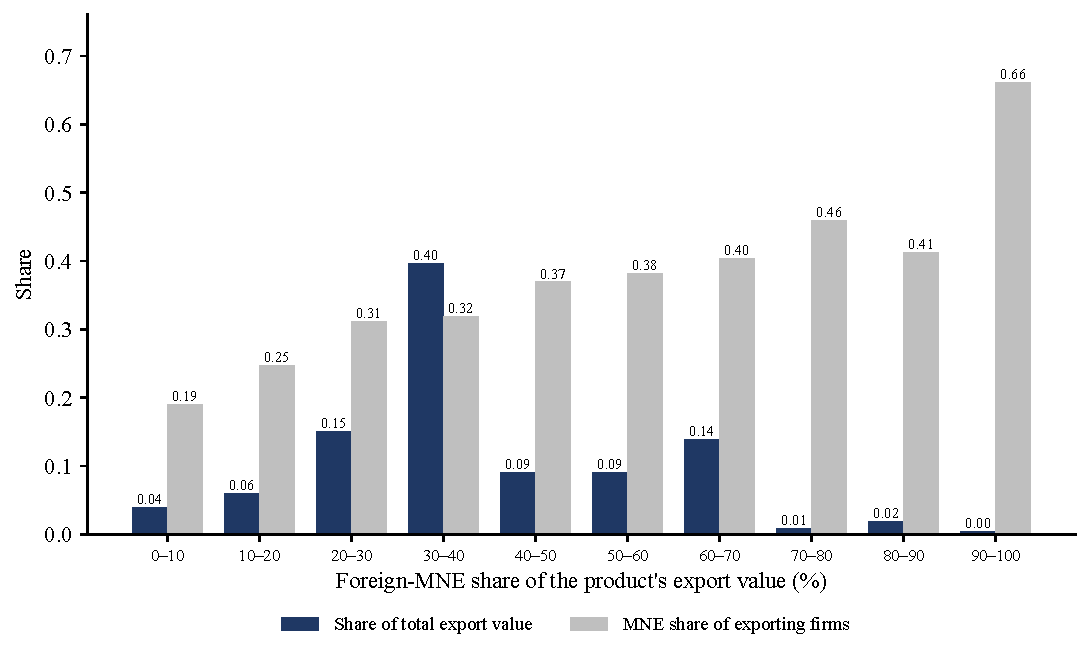
\includegraphics[width=0.85\textwidth,height=0.8\textheight,keepaspectratio]{figures/agro/fig_wp1f_foreign_share_distribution.pdf}%
  \par\vspace{2pt}%
  \parbox{0.92\textwidth}{\footnotesize %
  \textit{Notes:} Share of agricultural export value and MNE share of exporting firms, by the foreign-MNE share of each product's export value, 2012--2018.\\[3pt]%
  \srcnote}%
  \end{figure}

\subsection{Product Sophistication}\label{sec:ap_soph}


% ---- Figure: Multinational Share of Agricultural Exports, by Product Sophistication
\begin{figure}[H]\centering%
  \caption{Multinational Share of Agricultural Exports, by Product Sophistication}%
  \label{fig:ap_soph}%
  \begin{minipage}[t]{0.72\textwidth}\centering\textbf{Panel A. Product Complexity Index quintile}\\[2pt]%
  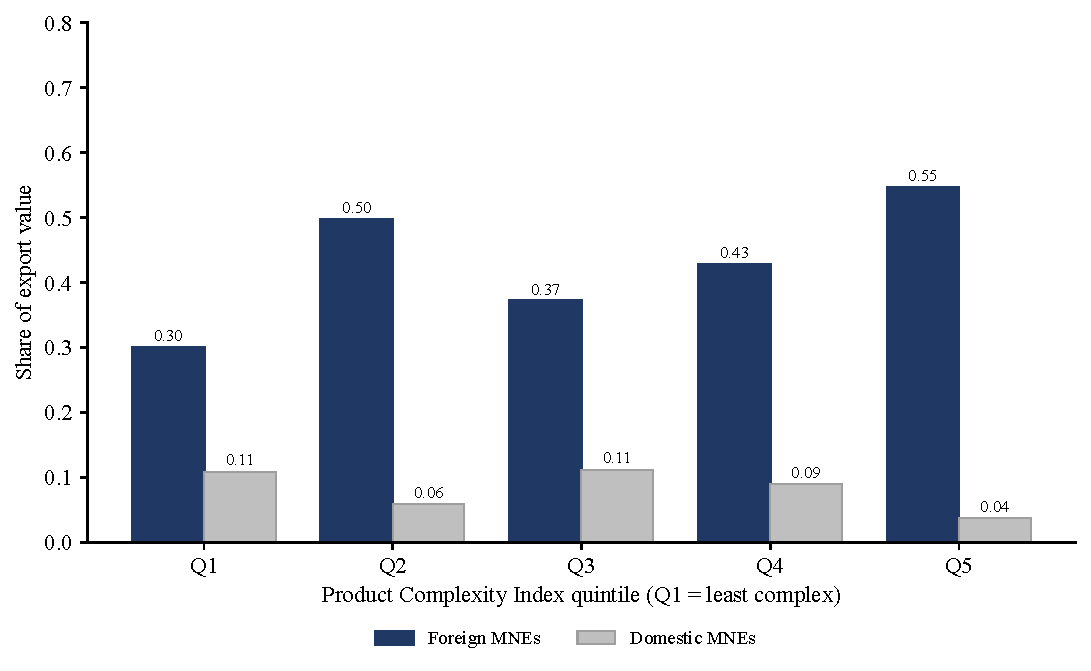
\includegraphics[width=\linewidth,height=0.38\textheight,keepaspectratio]{figures/agro/fig_wp0_fig2_pci.pdf}%
  \end{minipage}\\[8pt]%
  \begin{minipage}[t]{0.72\textwidth}\centering\textbf{Panel B. Lall (2000) technology class}\\[2pt]%
  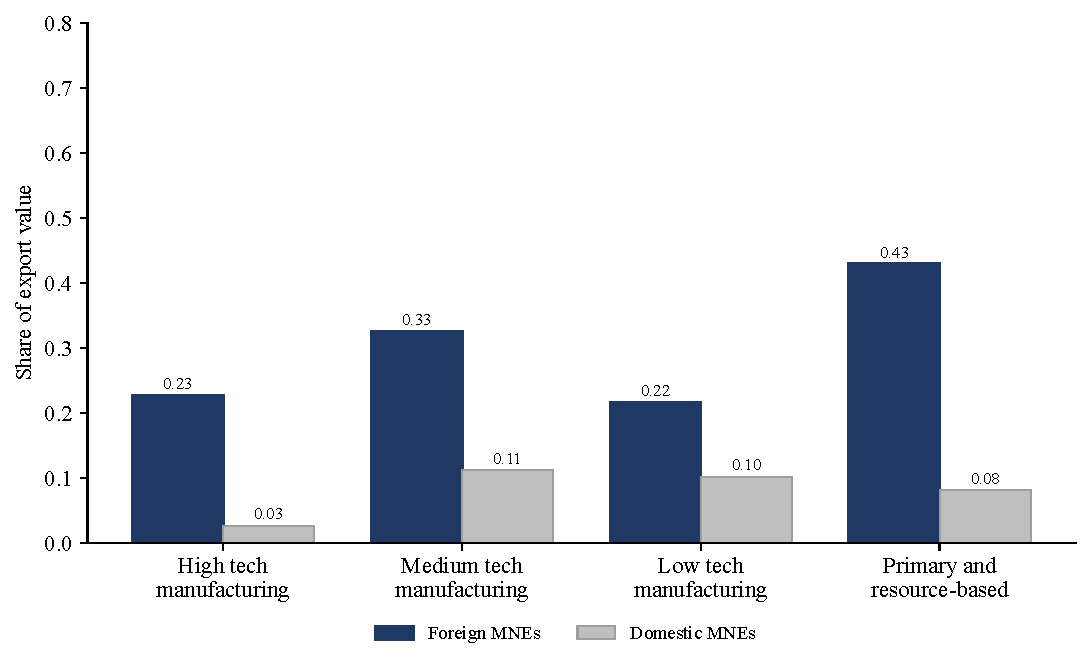
\includegraphics[width=\linewidth,height=0.38\textheight,keepaspectratio]{figures/agro/fig_wp0_fig3_lall.pdf}%
  \end{minipage}%
  \par\vspace{2pt}%
  \parbox{0.92\textwidth}{\footnotesize %
  \textit{Notes:} Shares of agricultural export value, 2012--2018 pooled. Panel A: quintiles of the Product Complexity Index of Hausmann and Hidalgo (2011), which ranks products by how diverse and advanced the countries that export them are (Q1 = least complex). Panel B: technology classes of Lall (2000): primary products, resource-based manufactures, and low-, medium- and high-technology manufactures.\\[3pt]%
  \srcnote}%
  \end{figure}

% ---- Table: Multinational Share of Agricultural Exports, by Rauch Product Class
\begin{table}[H]\centering\small%
  \caption{Multinational Share of Agricultural Exports, by Rauch Product Class}%
  \label{tab:ap_rauch}%
  \adjustbox{max width=\textwidth, max totalheight=0.8\textheight}{\begin{tabular}{lcccrr}
\toprule
Rauch (1999) class & Foreign & Domestic & All MNEs & Products & Value (US\$bn/yr) \\
\midrule
Differentiated & 0.432 & 0.081 & 0.513 & 166 & 7.7 \\
Reference-priced & 0.325 & 0.092 & 0.417 & 351 & 20.1 \\
Homogeneous (exchange) & 0.412 & 0.094 & 0.506 & 164 & 43.1 \\
\bottomrule
\end{tabular}
}%
  \par\vspace{3pt}%
  \begin{minipage}{0.95\textwidth}\footnotesize %
  \textit{Notes:} Shares of agricultural export value, 2012--2018 pooled. Rauch (1999) conservative classification: homogeneous goods are traded on organized exchanges, reference-priced goods have a price quoted in trade publications, and differentiated goods have neither. Values are annual averages over 2012--2018, in US\$ billion.\\[3pt]%
  \srcnote%
  \end{minipage}%
  \end{table}

% ---- Figure: Multinational Share of Agricultural Exports, by Rauch Product Class
\begin{figure}[H]\centering%
  \caption{Multinational Share of Agricultural Exports, by Rauch Product Class}%
  \label{fig:ap_rauch}%
  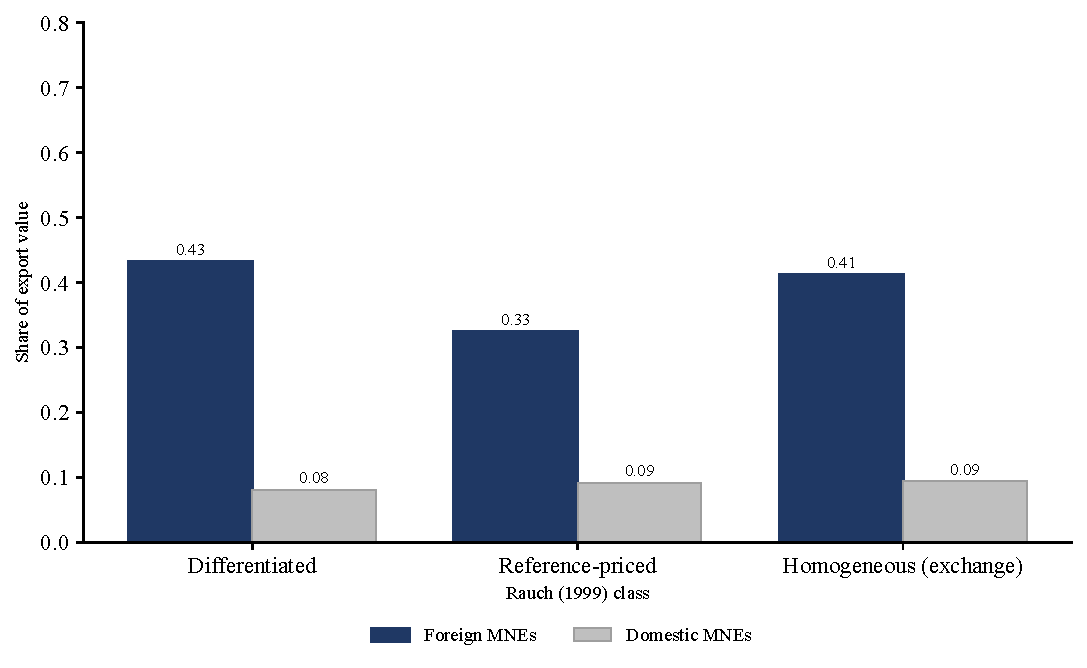
\includegraphics[width=0.7\textwidth,height=0.8\textheight,keepaspectratio]{figures/agro/fig_wp1b_rauch.pdf}%
  \par\vspace{2pt}%
  \parbox{0.92\textwidth}{\footnotesize %
  \textit{Notes:} Shares of agricultural export value, 2012--2018 pooled. Rauch (1999) conservative classification: homogeneous goods are traded on organized exchanges, reference-priced goods have a price quoted in trade publications, and differentiated goods have neither.\\[3pt]%
  \srcnote}%
  \end{figure}

% ---- Table: Multinational Share of Agricultural Exports, by End Use and Number of Products
\begin{table}[H]\centering\small%
  \caption{Multinational Share of Agricultural Exports, by End Use and Number of Products}%
  \label{tab:ap_bec2}%
  \adjustbox{max width=\textwidth, max totalheight=0.8\textheight}{\begin{tabular}{lcccrr}
\toprule
BEC end use & Foreign & Domestic & All MNEs & Products & Value (US\$bn/yr) \\
\midrule
Intermediate & 0.415 & 0.090 & 0.505 & 241 & 42.5 \\
Consumption & 0.362 & 0.091 & 0.452 & 451 & 29.6 \\
Capital & 0.173 & 0.016 & 0.189 & 3 & 0.0 \\
\bottomrule
\end{tabular}
}%
  \par\vspace{3pt}%
  \begin{minipage}{0.95\textwidth}\footnotesize %
  \textit{Notes:} Shares of agricultural export value, 2012--2018 pooled, by BEC Rev.\,4 end use; products without a BEC correspondence are excluded. Values are annual averages over 2012--2018, in US\$ billion.\\[3pt]%
  \srcnote%
  \end{minipage}%
  \end{table}

% ---- Table: Product Sophistication and Multinational Shares in Agriculture
\begin{table}[H]\centering\footnotesize%
  \caption{Product Sophistication and Multinational Shares in Agriculture}%
  \label{tab:ap_ladder}%
  \adjustbox{max width=\textwidth, max totalheight=0.8\textheight}{\begin{tabular}{lcccccc} \hline
 & \multicolumn{2}{c}{PCI} & \multicolumn{2}{c}{Lall} & \multicolumn{2}{c}{Rauch} \\
 & (1) & (2) & (3) & (4) & (5) & (6) \\ \hline
\multicolumn{7}{l}{\textit{Panel A. Dependent variable: share of all MNEs}} \\
Complexity (PCI) & 0.0679*** & 0.0555*** &  &  &  &  \\
 & (0.0072) & (0.0074) &  &  &  &  \\
Lall: high tech (vs primary and resource-based) &  &  & -0.2163*** & -0.2232*** &  &  \\
 &  &  & (0.0120) & (0.0118) &  &  \\
Lall: medium tech &  &  & -0.0424*** & -0.0484*** &  &  \\
 &  &  & (0.0073) & (0.0079) &  &  \\
Lall: low tech &  &  & -0.1859*** & -0.1650*** &  &  \\
 &  &  & (0.0395) & (0.0366) &  &  \\
Rauch: differentiated (vs homogeneous) &  &  &  &  & 0.0531*** & 0.0591*** \\
 &  &  &  &  & (0.0108) & (0.0121) \\
Rauch: reference-priced &  &  &  &  & -0.0342*** & -0.0259*** \\
 &  &  &  &  & (0.0083) & (0.0080) \\
Observations & 107,209 & 105,699 & 184,023 & 182,613 & 181,273 & 179,905 \\
\midrule
\multicolumn{7}{l}{\textit{Panel B. Dependent variable: share of foreign MNEs}} \\
Complexity (PCI) & 0.0560*** & 0.0495*** &  &  &  &  \\
 & (0.0079) & (0.0083) &  &  &  &  \\
Lall: high tech (vs primary and resource-based) &  &  & -0.1613*** & -0.1708*** &  &  \\
 &  &  & (0.0107) & (0.0110) &  &  \\
Lall: medium tech &  &  & -0.0695*** & -0.0748*** &  &  \\
 &  &  & (0.0080) & (0.0086) &  &  \\
Lall: low tech &  &  & -0.2005*** & -0.2016*** &  &  \\
 &  &  & (0.0206) & (0.0167) &  &  \\
Rauch: differentiated (vs homogeneous) &  &  &  &  & 0.0726*** & 0.0737*** \\
 &  &  &  &  & (0.0118) & (0.0130) \\
Rauch: reference-priced &  &  &  &  & -0.0334*** & -0.0253*** \\
 &  &  &  &  & (0.0084) & (0.0080) \\
Observations & 107,209 & 105,699 & 184,023 & 182,613 & 181,273 & 179,905 \\
\midrule
\multicolumn{7}{l}{\textit{Panel C. Dependent variable: share of domestic MNEs}} \\
Complexity (PCI) & 0.0119*** & 0.0060 &  &  &  &  \\
 & (0.0036) & (0.0039) &  &  &  &  \\
Lall: high tech (vs primary and resource-based) &  &  & -0.0551*** & -0.0524*** &  &  \\
 &  &  & (0.0061) & (0.0064) &  &  \\
Lall: medium tech &  &  & 0.0272*** & 0.0263*** &  &  \\
 &  &  & (0.0038) & (0.0039) &  &  \\
Lall: low tech &  &  & 0.0146 & 0.0366 &  &  \\
 &  &  & (0.0356) & (0.0380) &  &  \\
Rauch: differentiated (vs homogeneous) &  &  &  &  & -0.0195*** & -0.0146*** \\
 &  &  &  &  & (0.0050) & (0.0047) \\
Rauch: reference-priced &  &  &  &  & -0.0008 & -0.0006 \\
 &  &  &  &  & (0.0046) & (0.0049) \\
Observations & 107,209 & 105,699 & 184,023 & 182,613 & 181,273 & 179,905 \\
\hline
Origin $\times$ year and destination $\times$ year FE & $\checkmark$ &  & $\checkmark$ &  & $\checkmark$ &  \\
Origin $\times$ dest.\ $\times$ year FE &  & $\checkmark$ &  & $\checkmark$ &  & $\checkmark$ \\
\hline
\end{tabular}
}%
  \par\vspace{3pt}%
  \begin{minipage}{0.95\textwidth}\footnotesize %
  \textit{Notes:} Regression at the origin country, destination country, product and year level; agricultural products, 2012--2018. Dependent variable: share of export value shipped by each type of MNE. Omitted categories: primary and resource-based products (Lall) and homogeneous products (Rauch). Robust standard errors in parentheses. *** $p<0.01$, ** $p<0.05$, * $p<0.1$.\\[3pt]%
  \srcnote%
  \end{minipage}%
  \end{table}

% ---- Table: Multinational Share of Agricultural Exports, by Quintile of Each Sophistication Measure
\begin{table}[H]\centering\footnotesize%
  \caption{Multinational Share of Agricultural Exports, by Quintile of Each Sophistication Measure}%
  \label{tab:ap_quint}%
  \adjustbox{max width=\textwidth, max totalheight=0.8\textheight}{\begin{tabular}{lccccc|ccccc}
\toprule
 & \multicolumn{5}{c}{Foreign MNE share} & \multicolumn{5}{c}{Domestic MNE share} \\
Measure & Q1 & Q2 & Q3 & Q4 & Q5 & Q1 & Q2 & Q3 & Q4 & Q5 \\
\midrule
PCI & 0.30 & 0.50 & 0.37 & 0.43 & 0.55 & 0.11 & 0.06 & 0.11 & 0.09 & 0.04 \\
$|\sigma|$ FGO (2022) & 0.42 & 0.41 & 0.38 & 0.30 & 0.33 & 0.06 & 0.08 & 0.12 & 0.12 & 0.10 \\
$\sigma$ Broda--Weinstein & 0.37 & 0.34 & 0.44 & 0.49 & -- & 0.12 & 0.10 & 0.06 & 0.05 & -- \\
Upstreamness & 0.33 & 0.31 & 0.38 & 0.38 & 0.44 & 0.07 & 0.08 & 0.11 & 0.12 & 0.08 \\
Quality ladder & -- & -- & -- & -- & -- & -- & -- & -- & -- & -- \\
RHCI & 0.42 & 0.49 & 0.36 & 0.43 & 0.32 & 0.10 & 0.05 & 0.10 & 0.08 & 0.10 \\
\bottomrule
\end{tabular}
}%
  \par\vspace{3pt}%
  \begin{minipage}{0.95\textwidth}\footnotesize %
  \textit{Notes:} Shares of export value within each quintile of agricultural products, 2012--2018. --: fewer than 30 products carry the measure.\\[3pt]%
  \srcnote%
  \end{minipage}%
  \end{table}
\end{document}
